\documentclass[UTF8,fontset=windows,11pt]{ctexart}
\usepackage[a4paper,margin=2.35cm]{geometry}
\usepackage{amsmath,amssymb,bm,mathtools}
\usepackage{booktabs,longtable,array}
\usepackage{graphicx}
\graphicspath{{figures/v4/}}
\usepackage[section]{placeins}
\usepackage{xcolor}
\usepackage{enumitem}
\usepackage{algorithm}
\usepackage{algpseudocode}
\usepackage{amsthm}
\usepackage{caption}
\captionsetup{font=small,labelfont=bf,labelsep=quad,skip=6pt}
\setlength{\textfloatsep}{14pt plus 3pt minus 3pt}
\setlength{\floatsep}{12pt plus 2pt minus 2pt}
\renewcommand{\topfraction}{0.92}
\renewcommand{\bottomfraction}{0.85}
\renewcommand{\textfraction}{0.07}
\renewcommand{\floatpagefraction}{0.72}
\setcounter{topnumber}{3}
\setcounter{totalnumber}{5}
\raggedbottom
\ctexset{section={format=\Large\bfseries\raggedright},subsection={format=\large\bfseries\raggedright}}
\makeatletter
\renewcommand{\maketitle}{\begin{center}\vspace*{-1em}{\LARGE\bfseries\@title\par}\vspace{1em}\end{center}}
\makeatother
\usepackage{hyperref}
\usepackage{microtype}
\newcommand{\upcite}[1]{\textsuperscript{\cite{#1}}}
\floatname{algorithm}{算法}
\newtheorem{theorem}{定理}[section]
\newtheorem{proposition}[theorem]{命题}
\newtheorem{lemma}[theorem]{引理}
\newtheorem{corollary}[theorem]{推论}
\newtheorem{definition}[theorem]{定义}
\newcommand{\Sone}{\mathbb S^1}
\newcommand{\Ttwo}{\mathbb T^2}
\newcommand{\E}{\mathbb E}
\newcommand{\R}{\mathbb R}
\algrenewcommand\algorithmicrequire{\textbf{输入：}}
\algrenewcommand\algorithmicensure{\textbf{输出：}}
\algrenewcommand\algorithmicfor{\textbf{对于}}
\algrenewcommand\algorithmicdo{\textbf{执行}}
\algrenewcommand\algorithmicend{\textbf{结束}}
\algrenewcommand\algorithmicreturn{\textbf{返回}}
\hypersetup{colorlinks=true,linkcolor=black,citecolor=black,urlcolor=blue,
 pdftitle={间歇方位观测下异中心神经场的预测输入重建与配对评估},
 pdfsubject={异中心神经场集群运动与Kalman预测补偿},
 pdfkeywords={异中心表征；环形吸引子；集群运动；间歇观测；Kalman滤波},
 bookmarksnumbered=true}
\setlength{\parindent}{2em}
\setlength{\parskip}{0.12em}
\linespread{1.10}
\setlength{\emergencystretch}{1em}
\title{间歇方位观测下异中心神经场的\newline 预测输入重建与配对评估}
\author{}
\date{}
\begin{document}
\maketitle

\begin{abstract}
邻居方位的连续缺失会同时改变异中心神经场的输入幅值和方向结构。本文在已有环形神经场动力学上，构建历史方位预测到社会输入的重建接口，并区分输入重建与闭环响应。首先，将指数方位加权和作为低维经验描述量；在 $20$ 组随机几何、$240$ 个配对条件的留组交叉验证中，其局部纵向响应预测 RMSE 比总幅值基准低 $16.1\%$。其次，采用方位--角速度 Kalman 模型，并将近似方位后验通过周期核卷积映射为输入。理论分析给出指定后验下的条件均方重建性质、方向谐波衰减及以实际输入差为驱动的有限时间状态界。在五个开发种子的中心条件中，KF 均值输入相对最后方位保持的同状态输入误差降低 $61.8\%$；方位误差的优势则依赖汇总方式，逐种子 RMSE 均值降低 $26.4\%$，合并平方误差后的 RMSE 增高 $13.5\%$。三十种子配对闭环实验显示，补偿可在所测条件下降低相对无遮挡参考的偏差，但相对方位保持的增量随指标和缺失时长变化。当前协方差存在失配，结果属于固定身份、等权和脚本化缺失下的探索性证据，不构成普遍预测优势或集群稳定性保证。

\end{abstract}

\noindent\textbf{关键词：} 异中心表征；环形吸引子；集群运动；间歇观测；Kalman滤波；方位预测；不确定性传播

\section{引言}

局部感知约束是分布式集群运动的重要问题。有限视场下的多无人机控制需要协调邻居感知与排斥行为\upcite{Bai2024}，林下集群导航需要处理环境不确定性\upcite{Boldrer2026}，通信障碍也会影响集群凝聚\upcite{LiFlocking2024}。这些研究说明感知和信息可用性必须与交互机制共同考虑。本文聚焦一个更受限的模型问题：已关联邻居的方位连续缺失时，如何利用合法历史观测重建异中心神经场输入。

若按决策所依赖的信息和计算组织方式划分，多智能体协同控制可分为集中式与分布式两类。集中式方法汇集个体状态并统一计算控制指令，便于协调全局任务，但需要持续获取和传递群体信息；分布式方法则由各个体依据本地观测及可获得的邻居信息更新自身行为\upcite{OlfatiSaber2006}。对于需要持续协同运动的无人集群，后者能够将群体协调建立在局部交互之上，但其运动效果也取决于邻居信息的可获得性和表达方式。由局部交互产生有序集体运动的 flocking，因而成为研究这一问题的典型模型。

flocking 建模关注局部交互如何产生有序的集体运动。Reynolds 在1987年发表的 Boids 模型通过分离、对齐和凝聚三类局部行为模拟群体运动\upcite{Reynolds1987}；Vicsek 等人在1995年通过局部航向对齐建立自驱动粒子模型，研究集体运动的有序相变\upcite{Vicsek1995}；Olfati--Saber 于2006年将 flocking 写成分布式控制律，并建立相应的算法与理论分析框架\upcite{OlfatiSaber2006}。这些研究从行为规则和控制律出发描述群体运动。Salahshour 与 Couzin（2025）进一步从方位信息的神经表征出发，将邻居方位映射到环形吸引子网络，比较自我中心与异中心表征对集体运动的影响。本文采用其中神经场模型（neural field model）的异中心表征版本，后文简称“异中心神经场模型”\upcite{Salahshour2025}。该模型仅依靠邻居方位输入即可产生有序集体运动，为研究社会输入与群体运动的关系提供了具体机制。

在实际感知与通信过程中，遮挡和链路中断会使邻居方位观测间歇缺失。删除缺失邻居会同时改变总输入幅值与方位结构；保持最后一次观测则可能在群体转向时持续提供过期方向。因此，需要量化邻居信息对社会输入的作用，并利用历史方位重建缺失期间的方向输入。

间歇观测下的 Kalman 估计已有成熟基础。Sinopoli 等分析了线性高斯系统在随机观测到达下的估计协方差\upcite{Sinopoli2004}。本文沿用缺失时仅预测的递推结构，研究有限连续缺失期间的方位信息如何进入神经场，不将标准滤波递推或条件期望投影原理作为新的滤波理论。仅方位目标跟踪还可通过平台机动和坐标建模处理目标状态估计\upcite{Xiourouppa2025}；本文仅估计局部方位及其变化率，不由此推断二维位置可观测性。

本文考察三个相互关联但证据层级不同的问题：（1）加入相对朝向信息的经验标量，是否比总幅值更能描述局部神经场的纵向响应；（2）历史方位外推及后验卷积如何改变同一几何状态下的输入重建；（3）这些输入策略在共同检查点分叉后，如何改变相对无遮挡参考的群体统计量。前一问题采用静态局部回放，后两问题分别采用同状态回放与闭环配对仿真，三者不互相替代。

本文的工作包括：给出指数方位描述量的定义及探索性局部验证；建立新鲜观测直通、缺失边预测和输入有效性门控的统一接口；推导该接口在指定后验下的重建性质，并报告均值误差、协方差失配、输入误差和闭环偏差。与原始异中心模型相比，新增内容集中于缺失观测的输入接口及其受控评价；原神经场动力学保持不变。

\section{问题描述}

\subsection{状态、观测与研究目标}

考虑 $N$ 个智能体在边长 $L$ 的二维周期区域内运动。每个智能体 $i$ 具有物理状态
\begin{equation}
 (q_i(k),\phi_i(k)),
\end{equation}
其中 $q_i(k)=[x_i(k),y_i(k)]^\top$ 是位置，$\phi_i(k)$ 是世界坐标系中的自身朝向。每个智能体同时维护一个包含 $M$ 个方向单元的环形神经场状态 $u_i(k)\in\mathbb R^M$ 和固定方向偏好
\begin{equation}
 \alpha_m=\frac{2\pi m}{M}+\phi_{i,0},\qquad m=0,\ldots,M-1,
\end{equation}
其中 $\phi_{i,0}$ 是初始化方向偏移。该表示是异中心的，即神经元方向固定在共同世界坐标系中，不随智能体自身朝向旋转。

智能体不能直接获得邻居位置，也不具有距离传感器。对于每条有向邻居边 $(i,j)$，传感器可能输出机体坐标系中的方位
\begin{equation}
 z^b_{ij}(k)=
 \operatorname{wrap}\left(\theta_{ij}(k)-\phi_i(k)+\nu_{ij}(k)\right),
\end{equation}
其中 $\theta_{ij}(k)$ 是邻居的世界方位，$\nu_{ij}(k)\sim\mathcal N(0,R)$ 是测量噪声。定义观测指示量
\begin{equation}
 \delta_{ij}(k)=
 \begin{cases}
 1, & \text{第 $k$ 步获得邻居 $j$ 的新鲜方位},\\
 0, & \text{观测缺失或通信中断}.
 \end{cases}
\end{equation}
已知自身朝向时，可将测量转换到世界坐标系：
\begin{equation}
 z_{ij}(k)=\operatorname{wrap}(z^b_{ij}(k)+\phi_i(k)).
\end{equation}

本文的问题可以描述为：在间歇方位观测条件下，利用截至当前时刻的观测历史构造因果预测与输入重建接口，在缺失期间延续邻居方向信息，并评价相对无遮挡参考的有序度与凝聚统计偏差。邻居真值用于离线评价，控制输入由观测及预测构成。

该问题的输入和输出如表~\ref{tab:problem_io} 所示。

\begin{table}[!tbp]
 \centering
 \small
 \caption{问题描述中的控制器输入与输出}
 \label{tab:problem_io}
 \begin{tabular}{>{\raggedright\arraybackslash}p{0.16\linewidth}
                 >{\raggedright\arraybackslash}p{0.37\linewidth}
                 >{\raggedright\arraybackslash}p{0.35\linewidth}}
 \toprule
 层级 & 输入 & 输出\\
 \midrule
 传感器层 &
 自身朝向 $\phi_i(k)$；已关联邻居编号 $j$；新鲜方位 $z_{ij}(k)$；观测指示量 $\delta_{ij}(k)$ &
 经过噪声和遮挡处理后的方位观测\\
 预测层 &
 当前边历史观测 $z_{ij}(0:k)$；上一步估计 $\hat x_{ij}(k-1)$ 和协方差 $P_{ij}(k-1)$ &
 预测方位均值 $\mu_{ij}(k)$；方位方差 $V_{ij}(k)$；轨迹有效指示量 $m_{ij}(k)$\\
 神经场层 &
 神经元方向 $\alpha_m$；神经场状态 $u_i(k)$；预测方位及方差 &
 外部社会输入 $I_i(k)$；更新后的神经活动 $u_i(k+1)$\\
 运动层 &
 正神经活动 $a_{im}(k+1)$；速度尺度 $v_s$ &
 运动速度 $v_i(k)$；更新位置 $q_i(k+1)$\\
 \bottomrule
 \end{tabular}
\end{table}

令 $\mathcal Z_i(0:k)=\{(j,z_{ij}(t),\delta_{ij}(t)):t\le k\}$ 表示智能体 $i$ 截至第 $k$ 步的全部可用观测历史。同状态输入估计的理想目标可形式化为
\begin{equation}
 \min_{\Pi}\ \mathbb E\left[
 \left\|I_i^{\mathrm{true}}(k)-\Pi(\mathcal Z_i(0:k),u_i(k);\Theta)\right\|_2^2
 \right],
\end{equation}
其中 $\Pi$ 是满足因果性约束的预测输入重建接口，$\Theta$ 是滤波器参数，$I_i^{\mathrm{true}}$ 是如果所有邻居方位均新鲜时异中心神经场模型将获得的社会输入。该目标依赖真实条件分布，本文仅以近似后验构造输入，不求解一般闭环最优控制问题。闭环评价报告 GO、LO 与凝聚距离相对参考的偏差；这些量不等价于任务完成、转向跟随精度或恢复时间。

本文进一步假设：

\begin{enumerate}[label=(\arabic*)]
 \item 邻居编号已经正确关联，不考虑错误匹配和轨迹交换；
 \item 自身朝向 $\phi_i(k)$ 已知，不考虑自身朝向估计误差；
 \item 传感器只提供方位，不提供距离，本研究不引入未经可观测性论证的二维位置--速度估计；
 \item 预测接口使用截至当前时刻的历史观测，隐藏真值和未来状态用于离线评价。
\end{enumerate}

\subsection{异中心神经场模型的求解}

本节给出 Salahshour 与 Couzin（2025）神经场模型的异中心表征版本\upcite{Salahshour2025}的求解过程。该模型使用连续可得的邻居方位和全邻居交互。对每个智能体 $i$，其社会邻居集合固定为
\begin{equation}
 \mathcal B_i=\{j\in\{1,\ldots,N\}:j\ne i\}.
\end{equation}
对邻居 $j$，采用周期区域中的最小镜像差分
\begin{equation}
 r_{ij}(k)=q_j(k)-q_i(k)-L\operatorname{round}\left(\frac{q_j(k)-q_i(k)}{L}\right).
\end{equation}
其真实世界方位为
\begin{equation}
 \theta_{ij}(k)=\operatorname{atan2}(r_{ij,y}(k),r_{ij,x}(k)).
\end{equation}
定义圆周角距离
\begin{equation}
 d_{\mathbb S^1}(a,b)=\left|\operatorname{wrap}(a-b)\right|,
\quad \operatorname{wrap}(x)=\operatorname{mod}(x+\pi,2\pi)-\pi.
\end{equation}

完整新鲜社会输入为
\begin{equation}
 I^{\mathrm{soc}}_{im}(k)=h_0\sum_{j\in\mathcal B_i}
 g_\sigma\left(\alpha_m-\theta_{ij}(k)\right),
 \quad h_0=\frac{h_t}{N},
\end{equation}
其中
\begin{equation}
 g_\sigma(x)=\exp\left[-\frac{d_{\mathbb S^1}^2(x,0)}{2\sigma_s^2}\right].
\end{equation}
这里 $\mathcal B_i$ 是固定全邻居集合。实际幅值总和为 $(N-1)h_t/N$。

令 $d_{mn}=d_{\mathbb S^1}(2\pi m/M,2\pi n/M)$。环形连接矩阵与神经场更新分别为
\begin{equation}
 W_{mn}=\cos\left[\pi\left(\frac{d_{mn}}{\pi}\right)^\zeta\right],
\end{equation}
\begin{equation}
 u_i(k+1)=u_i(k)+\Delta t\left[-u_i(k)+\frac{1}{M}W\tanh(\beta u_i(k))-h_b\bm 1+I_i(k)\right].
\end{equation}
神经场内部使用未截断的 $\tanh$。运动解码时定义正活动
\begin{equation}
 a_{im}(k+1)=\max\{\tanh(\beta u_{im}(k+1)),0\},
\end{equation}
并令
\begin{equation}
 c_i(k+1)=\sum_{m=0}^{M-1}a_{im}(k+1)e^{\mathrm i\alpha_m},
\quad
 v_i(k)=v_s[\Re c_i(k+1),\Im c_i(k+1)]^\top,
\end{equation}
\begin{equation}
 q_i(k+1)=\operatorname{mod}(q_i(k)+\Delta t v_i(k),L).
\end{equation}
这里 $v_i(k)$ 表示从第 $k$ 步到第 $k+1$ 步的区间速度，由更新后的 $u_i(k+1)$ 解码。若 $|\Re c_i(k+1)|+|\Im c_i(k+1)|\ge10^{-9}$，令 $\phi_i(k+1)=\arg c_i(k+1)$；否则保留上一朝向。因此 $v_s$ 是速度尺度而不是恒定速度。单环活动集中度定义为
\begin{equation}
 \chi_i(k+1)=\frac{|c_i(k+1)|}{\sum_m a_{im}(k+1)+\varepsilon}.
\end{equation}

该环形连接和方向活动表示沿用原模型，并与头方向细胞群的周期朝向表征有关\upcite{Zhang1996}。本文不将这一生物启发机制直接等同于可部署飞行控制器。

异中心神经场模型的完整求解流程见算法~\ref{alg:original_model}。

\begin{algorithm}[!tbp]
 \caption{异中心神经场模型的求解流程}
 \label{alg:original_model}
 \begin{algorithmic}[1]
 \Require 模型参数 $N,M,L,\Delta t,v_s,\beta,\sigma_s,h_t,h_b,\zeta$
 \Require 初始状态 $q_i(0)$、$\phi_i(0)$、$u_i(0)$，或用于随机初始化的随机种子
 \Ensure 轨迹 $\{q_i(k)\}_{i=1,k=0}^{N,K}$、神经状态 $\{u_i(k)\}_{i=1,k=0}^{N,K}$ 和社会输入历史 $\{I_i(k)\}$
 \State 初始化
 $q_i(0)\sim\mathcal U([0,L)^2)$，
 $\phi_i(0)\sim\mathcal U(0,2\pi)$，
 $u_i(0)=0.1\epsilon_i$，
 $\epsilon_i\sim\mathcal N(0,I_M)$
 \State 设置 $\alpha_m=2\pi m/M+\phi_i(0)$，并在后续时刻保持固定
 \For{$k=0,1,\ldots,K-1$}
  \For{所有 $i=1,2,\ldots,N$，并行}
   \State $\mathcal B_i\leftarrow\{j:j\ne i\}$；$I_i^{\mathrm{soc}}(k)\leftarrow\mathbf 0$
   \For{$j\in\mathcal B_i$}
    \State 计算周期差分 $r_{ij}(k)$ 和世界方位 $\theta_{ij}(k)$
    \State 将邻居方位累加到圆周高斯输入 $I^{\mathrm{soc}}_{im}(k)$
   \EndFor
   \State $I_i(k)\leftarrow I^{\mathrm{soc}}_{i}(k)$
   \State $u_i(k+1)\leftarrow
   u_i(k)+\Delta t\left[-u_i(k)+\frac{1}{M}W\tanh(\beta u_i(k))-h_b\mathbf 1+I_i(k)\right]$
   \State 从更新后的神经状态计算 $a_{im}(k+1)$ 和 $c_i(k+1)$
   \State 解码速度 $v_i(k)=v_s[\Re c_i(k+1),\Im c_i(k+1)]^\top$
  \EndFor
  \For{所有 $i=1,2,\ldots,N$，并行}
   \State 更新位置 $q_i(k+1)=\operatorname{mod}(q_i(k)+\Delta t v_i(k),L)$
  \EndFor
 \EndFor
 \State \Return $\{q_i(k)\}$、$\{u_i(k)\}$、$\{I_i(k)\}$
 \end{algorithmic}
\end{algorithm}

算法~\ref{alg:original_model} 对应异中心神经场模型的全邻居版本，其中所有个体均使用同一时刻的位置计算输入，并在该时间步结束时同步更新。GO、LO、凝聚距离和活动集中度等指标不参与状态更新，而是由返回的轨迹和神经状态离线计算。

本文以全邻居、等权交互的异中心神经场模型为基础。邻居选择还可能受视觉线索\upcite{Krongauz2024}、注意力机制\upcite{Li2024}和选择性交互\upcite{Xue2025}影响；为拆分数量、强度和方位的作用，下面对给定邻居集合建立统一的输入表征。


\subsection{邻居社会输入的经验量化模型}
\label{sec:social_input_model}

\subsubsection{方位编码与单邻居输入}

沿用 Salahshour 与 Couzin 的异中心方位编码\upcite{Salahshour2025}，$\theta_{ij}(k)$ 表示从智能体 $i$ 指向邻居 $j$ 的方位，$\phi_i(k)$ 表示自身运动朝向，二者均在同一固定参照系下表达。本文取机体前向轴与运动朝向一致，此时无噪声机体方位满足 $z^b_{ij}(k)=\operatorname{wrap}(\theta_{ij}(k)-\phi_i(k))$。定义自身朝向和邻居方位的单位向量
\begin{equation}
 e_i(k)=\begin{bmatrix}\cos\phi_i(k)\\\sin\phi_i(k)\end{bmatrix},
 \qquad
 b_{ij}(k)=\begin{bmatrix}\cos\theta_{ij}(k)\\\sin\theta_{ij}(k)\end{bmatrix}.
\end{equation}
其中 $b_{ij}$ 描述邻居相对自身的位置方位。单位内积 $e_i^\top b_{ij}=\cos(\theta_{ij}-\phi_i)$ 表示该方位与自身朝向的接近程度，计算时只需邻居方位和自身朝向。

本文选取指数余弦函数作为经验方位权重
\begin{equation}
 f_\kappa(\psi)
 =\frac{\exp(\kappa\cos\psi)}{\exp(\kappa)}
 =\exp\!\left[\kappa(\cos\psi-1)\right],\qquad\kappa>0.
 \label{eq:exponential_bearing_weight}
\end{equation}
参数 $\kappa$ 控制方位权重的集中程度，$\kappa$ 越大，权重越集中于正前方；分母 $\exp(\kappa)$ 将最大权重归一化为 $1$。本轮探索固定 $\kappa=1$，未证明该取值最优；此时 $f_1(\psi)=\exp(\cos\psi)/e$。

令 $w_{ij}(k)\geq0$ 为邻居 $j$ 对神经场的实际输入强度，即方向高斯核前的系数；等权设置取 $w_{ij}=h_0$。单邻居社会输入定义为
\begin{equation}
 \boxed{s_{ij}(k)=w_{ij}(k)f_\kappa\!\left(\theta_{ij}(k)-\phi_i(k)\right).}
 \label{eq:single_social_input}
\end{equation}
该量将输入强度与方位权重相乘，使接近自身当前运动朝向的邻居方位具有更高权重。当 $\kappa=1$ 时，正前方、正侧方和正后方邻居分别贡献 $w_{ij}$、$e^{-1}w_{ij}\approx0.368w_{ij}$ 和 $e^{-2}w_{ij}\approx0.135w_{ij}$；具有正输入强度的邻居在各个方位均保留正贡献。

\subsubsection{总社会输入与因素分解}

对当前参与输入的邻居集合 $\mathcal N_i(k)$ 求和，得到总社会输入经验量化公式
\begin{equation}
 \boxed{\displaystyle S_i(k)=\sum_{j\in\mathcal N_i(k)}w_{ij}(k)
 \exp\!\left\{\kappa\left[\cos(\theta_{ij}(k)-\phi_i(k))-1\right]\right\}.}
 \label{eq:total_social_input}
\end{equation}
邻居数量通过求和项数体现。定义邻居数 $n_i=|\mathcal N_i|$、总输入幅值 $A_i$、平均单邻居强度 $\bar w_i$ 和归一化方位权重 $C_i$：
\begin{align}
 A_i&=\sum_{j\in\mathcal N_i}w_{ij},\qquad
 \bar w_i=\frac{A_i}{n_i},\\
 C_i&=\sum_{j\in\mathcal N_i}\frac{w_{ij}}{A_i}
 f_\kappa(\theta_{ij}-\phi_i),\qquad e^{-2\kappa}\leq C_i\leq1.
\end{align}
在 $n_i>0$、$A_i>0$ 时，式~\eqref{eq:total_social_input} 可写为
\begin{equation}
 \boxed{S_i=A_iC_i=n_i\bar w_iC_i.}
 \label{eq:social_factorization}
\end{equation}
无有效输入时取 $S_i=0$、$C_i=0$。总量 $S_i$ 保留邻居数量和强度的累加作用，归一化量 $C_i$ 描述给定总幅值下的方位加权结构。固定单邻居强度和方位加权结构时，增加邻居数使 $S_i$ 线性增加；固定邻居数和方位时，整体放大输入强度使 $S_i$ 同比例缩放；固定总幅值时，方位变化通过 $C_i$ 改变 $S_i$。

群体仿真由完整的社会输入场驱动神经活动：
\begin{equation}
 I_i^{\mathrm{soc}}(\alpha,k)=\sum_{j\in\mathcal N_i(k)}w_{ij}(k)
 g_\sigma(\alpha-\theta_{ij}(k)).
\end{equation}
$A_i$ 是核系数之和，其与输入场积分之间的比例由核宽度决定；$S_i$ 对邻居输入按相对自身朝向的方位进行加权，表征数量、强度和方位的共同作用。实验以总幅值 $A_i$ 为基准，比较加入方位权重后的 $S_i$ 对局部神经场运动响应的解释能力。完整输入场仍用于驱动神经活动，经验量 $S_i$ 用于描述和分析输入。$S_i$ 不是输入场的充分统计量：例如相对方位 $+\psi$ 与 $-\psi$ 给出相同指数权重，却一般产生不同的横向运动。因而 $S_i$ 不能完整表征左右方向、多峰结构或网络连通性；$S_i=n_i\bar w_iC_i$ 是定义的代数分解，须与独立动力学证据区分。

\subsection{间歇观测下的社会输入变化与补偿需求}

异中心神经场模型使用连续可得的邻居方位输入。遮挡或通信中断会改变输入的幅值与方位结构，本文利用第~\ref{sec:social_input_model} 节的经验模型量化这些变化，并据此组织预测补偿需求。

\paragraph{社会输入缺失}
若直接删除缺失邻居，则
\begin{equation}
 I_i^{\mathrm{drop}}(k)=
 h_0\sum_{j\in\mathcal B_i(k)}\delta_{ij}(k)
 g_\sigma(\alpha_m-\theta_{ij}(k)).
\end{equation}
删除输入同时降低输入总幅值并改变方位覆盖，使神经场活动的强度和方向分布随剩余邻居发生变化。

\paragraph{过期方位造成错误峰}
若保持最后一次观测方位，则输入幅值可以维持，但方向可能已经过期：
\begin{equation}
 \hat\theta_{ij}(k)=z_{ij}(k_{\mathrm{last}}),
\quad k-k_{\mathrm{last}}>0.
\end{equation}
在群体转向时，过期方位会把神经活动峰持续固定在旧方向，形成“幽灵邻居输入”，可能造成方向响应滞后；其大小需由配对数据评价。

\paragraph{缺失信息的量化分解}

在同一时刻、以同一自身朝向为参考，记完整新鲜输入的幅值与归一化方位权重为 $A_i$、$C_i$，实际可用或重建输入的对应量为 $\widehat A_i$、$\widehat C_i$，则社会输入差异为
\begin{equation}
 \Delta S_i=S_i-\widehat S_i
 =(A_i-\widehat A_i)C_i
 +\widehat A_i(C_i-\widehat C_i).
 \label{eq:missing_input_decomposition}
\end{equation}
第一项描述总幅值变化的贡献，第二项描述归一化方位权重变化的贡献。删除输入时，缺失集合 $\mathcal H_i$ 造成的社会输入损失为
\begin{equation}
 \Delta S_i^{\mathrm{drop}}=
 \sum_{j\in\mathcal H_i}w_{ij}f_\kappa(\theta_{ij}-\phi_i)\geq0.
\end{equation}
保持旧方位时，输入幅值维持为 $A_i$，差异来自当前方位与旧方位的指数权重变化。以 $|\Delta S_i|$ 衡量社会输入量化误差，可将缺失邻居数、损失强度和方位变化连接到同一个可计算量；幅值项和方位项分别保留符号，用于辨别两种变化的作用方向。

\paragraph{方位状态与局部可观测性}
传感器提供邻居方位，局部预测状态据此选为方位及其时间变化率。连续不同时刻的方位观测用于识别局部角速度，自身朝向用于将观测转换至异中心参照系。

\paragraph{轨迹生命周期和数据关联问题}
实际跟踪系统需要区分暂时缺失和目标离开。本文固定邻居身份与真实存在性，仅用观测年龄和预测方差决定是否继续注入输入；不估计目标存在概率，也不实现数据关联或轨迹生灭。超限停止输入后仍保存滤波状态，恢复观测时继续更新。

\paragraph{转向响应评价}
群体进入直线运动后，既有航向惯性可维持较高 GO。本文设置遮挡前受控转向，激发邻居方位的时间变化，并报告相对无遮挡控制的 GO、LO 和凝聚距离偏差；这些指标不能单独衡量目标航向跟踪。

\paragraph{近距离风险诊断}
异中心神经场模型通过方位输入组织运动。本文以最小距离和危险接近比例诊断近距离风险，并将其与有序度和凝聚恢复分别评价；显式避碰约束作为后续控制扩展。

\section{间歇方位观测下的Kalman预测与神经场输入补偿}

邻居方位观测的间歇缺失会减少神经场的社会输入，并改变其方向结构。为在有限缺失窗口内延续已观测邻居的方向信息，本文建立由方位状态估计、缺失期间预测和神经场输入重建组成的补偿方法。每个智能体独立维护其已跟踪邻居的方位--方位角速度状态：观测到达时执行 Kalman 更新，观测缺失时保留模型预测，并将预测均值及协方差映射为神经场的周期方向输入。

\subsection{方法概述与观测模型}
设 $\delta_{ij}(k)\in\{0,1\}$ 表示观测是否新鲜到达。若传感器在机体坐标系中输出方位，且自身世界朝向 $\phi_i(k)$ 已知，则
\begin{equation}
 z^b_{ij}(k)=\operatorname{wrap}(\theta_{ij}(k)-\phi_i(k)+\nu_{ij}(k)),
\end{equation}
\begin{equation}
 z_{ij}(k)=\operatorname{wrap}(z^b_{ij}(k)+\phi_i(k)),
 \quad \nu_{ij}(k)\sim\mathcal N(0,R).
\end{equation}
仅当 $\delta_{ij}(k)=1$ 时执行测量更新。本文假设邻居目标编号正确，尚不处理数据关联错误和自身朝向误差。

\subsection{方位状态预测与测量更新}
\subsubsection{方位--方位角速度状态与阻尼扩展}
由于没有距离观测，定义局部展开角状态
\begin{equation}
 x_{ij}(k)=\begin{bmatrix}\vartheta_{ij}(k)\\ \omega_{ij}(k)\end{bmatrix},
 \quad \theta_{ij}(k)=\operatorname{wrap}(\vartheta_{ij}(k)),
\end{equation}
其中 $\vartheta_{ij}(k)$ 是局部展开角，$\theta_{ij}(k)$ 是其对应的圆周方位，$\omega_{ij}(k)$ 是邻居相对于观测者的方位角速度，并非邻居自身航向的角速度。基础模型采用局部常角速度假设
\begin{equation}
 x_{ij}(k+1)=F x_{ij}(k)+\eta_{ij}(k),
 \quad F=\begin{bmatrix}1&\Delta t\\0&1\end{bmatrix},
\end{equation}
\begin{equation}
 Q=q_\omega\begin{bmatrix}(\Delta t)^3/3&(\Delta t)^2/2\\(\Delta t)^2/2&\Delta t\end{bmatrix},
 \quad z_{ij}(k)=\operatorname{wrap}(Hx_{ij}(k)+\nu_{ij}(k)),\quad H=\begin{bmatrix}1&0\end{bmatrix}.
\end{equation}
其中过程噪声 $\eta_{ij}\sim\mathcal N(0,Q)$，与输入权重 $w_{ij}$ 区分。为减弱过期角速度的持续外推，进一步采用阻尼模型作为对照；是否改善误差由实验决定。令
$\rho=\exp(-\Delta t/\tau)$，其中 $\tau$ 为角速度相关时间，则
\begin{equation}
 x_{ij}(k+1)=F_{\mathrm{GM}}x_{ij}(k)+\eta_{ij}(k),
 \quad
 F_{\mathrm{GM}}=\begin{bmatrix}1&\tau(1-\rho)\\0&\rho\end{bmatrix},
\end{equation}
\begin{equation}
 Q_{\mathrm{GM}}=q_\omega
 \begin{bmatrix}
 \tau^2\Delta t-\tau^3\left(2(1-\rho)-\frac{1-\rho^2}{2}\right)
 & \frac{\tau^2(1-\rho)^2}{2}\\[2mm]
 \frac{\tau^2(1-\rho)^2}{2}
 & \frac{\tau(1-\rho^2)}{2}
 \end{bmatrix}.
\end{equation}
当 $\tau\to\infty$ 时，该模型退化为常角速度模型；当 $\tau$ 较小时，角速度预测向零衰减，从而降低长时间外推对过期角速度的依赖。上述模型只预测方位，不恢复邻居的二维位置或速度。

\subsubsection{初始化、预测与更新}
首次收到目标观测时初始化
\begin{equation}
 \hat x_{ij}(k)=\begin{bmatrix}z_{ij}(k)\\0\end{bmatrix},
 \quad P_{ij}(k)=\operatorname{diag}(R,P_{\omega,0}).
\end{equation}
对已初始化轨迹先执行
\begin{equation}
 \hat x^-_{ij}(k)=F\hat x_{ij}(k-1),\qquad
 P^-_{ij}(k)=FP_{ij}(k-1)F^\top+Q.
\end{equation}
当 $\delta_{ij}(k)=1$ 时，计算圆周创新
\begin{equation}
 e_{ij}(k)=\operatorname{wrap}\left(z_{ij}(k)-H\hat x^-_{ij}(k)\right),
\end{equation}
\begin{equation}
 S_{ij}=HP^-_{ij}H^\top+R,\quad K_{ij}=P^-_{ij}H^\top S_{ij}^{-1},
\end{equation}
\begin{equation}
 \hat x_{ij}(k)=\hat x^-_{ij}(k)+K_{ij}e_{ij}(k),
\end{equation}
\begin{equation}
 P_{ij}(k)=(I-K_{ij}H)P^-_{ij}(k)(I-K_{ij}H)^\top+K_{ij}RK_{ij}^\top.
\end{equation}
上述创新选择最接近预测均值的局部展开分支。普通高斯 KF 不自动抑制离群观测，本文未实施鲁棒更新。

当 $\delta_{ij}(k)=0$ 时仅保留预测值\upcite{Sinopoli2004}。观测年龄 $a_{ij}$ 在获得新鲜观测时归零，缺失时增加 $\Delta t$。扩展闭环批次在 $a_{ij}>\tau_{\max}$ 时停止缺失边输入；预测分支还要求 $P_{11,ij}\le P_{11,\max}$。停止注入不删除滤波状态，恢复观测后继续测量更新。hold 只受年龄门限约束，fresh-drop 不注入缺失边。记 $m_{ij}$ 为输入激活标记，它与轨迹是否存储、观测是否新鲜是三个不同概念。

观测矩阵为
\begin{equation}
 \mathcal O=\begin{bmatrix}H\\HF\end{bmatrix}=\begin{bmatrix}1&0\\1&\Delta t\end{bmatrix}.
\end{equation}
当 $\Delta t\ne0$ 时，$\det\mathcal O=\Delta t\ne0$。该秩条件仅说明选定展开分支下二状态代理模型的局部可观测性；单次观测不能识别角速度，跨采样间隔的角度混叠也不能由秩条件排除。该模型不涉及距离及二维位置的可观测性。

\subsection{不确定性感知神经场输入}

\subsubsection{预测均值输入}
定义
\begin{equation}
 \mu_{ij}(k)=H\hat x_{ij}(k),\quad V_{ij}(k)=HP_{ij}(k)H^\top.
\end{equation}
在给定已激活预测集合上，理想的纯预测均值输入为
\begin{equation}
 I^{\mathrm{mean}}_{im}(k)=h_0\sum_jm_{ij}(k)
 g_\sigma(\alpha_m-\mu_{ij}(k)),
\end{equation}
其中 $g_\sigma$ 为第~2.2 节定义的圆周高斯核，$\delta_{ij}$ 控制是否更新滤波器，$m_{ij}$ 控制预测轨迹是否继续注入神经场。实际各批次均使新鲜边直接使用当前测量，同时更新预测器；缺失边使用缓存权重。均值模式的混合输入为
\begin{equation}
 I^{\mathrm{mix}}_{im}(k)
 =\sum_{j\in\mathcal F_i(k)}w_{ij}(k)g_\sigma(\alpha_m-z_{ij}(k))
 +\sum_{j\in\mathcal H_i(k)}w_{ij}(k_{\mathrm{last}})
 g_\sigma(\alpha_m-\mu_{ij}(k)),
 \label{eq:pilot_causal_input}
\end{equation}
其中 $\mathcal F_i$ 为新鲜观测集合，$\mathcal H_i$ 为已经初始化、当前缺失且允许注入的邻居集合。新鲜观测既驱动当前输入，也更新预测器；缺失边通过历史观测形成的状态外推继续提供方向输入。

\subsubsection{协方差传播与周期卷积}
在局部高斯近似下，以 wrapped normal 分布近似方位后验
\begin{equation}
 \Theta_{ij}(k)\mid\mathcal Z_i(0:k)\sim\mathrm{WN}(\mu_{ij}(k),V_{ij}(k)).
\end{equation}
将社会输入定义为方位核的条件期望：
\begin{equation}
 \bar g_\sigma(x;V)=\int_{-\pi}^{\pi}g_\sigma(x-\epsilon)p_{\mathrm{WN}}(\epsilon;0,V)\,d\epsilon,
\end{equation}
\begin{equation}
 I^{\mathrm{unc}}_{im}(k)=h_0\sum_jm_{ij}(k)\bar g_\sigma(\alpha_m-\mu_{ij}(k);V_{ij}(k)).
\end{equation}

令
\begin{equation}
 c_n=\frac{1}{2\pi}\int_{-\pi}^{\pi}g_\sigma(x)e^{-\mathrm inx}\,dx,
\end{equation}
则周期卷积的 Fourier 形式为
\begin{equation}
 \bar g_\sigma(x;V)=\sum_{n=-\infty}^{\infty}c_n e^{-n^2V/2}e^{\mathrm inx}.
\end{equation}
因此第 $n$ 阶方向信息保留比例为 $e^{-n^2V/2}$，一阶方向信息保留比例为
\begin{equation}
 \gamma(V)=e^{-V/2}.
\end{equation}
当 $V$ 增大时，输入方向结构变宽并趋向均匀背景，零阶 Fourier 分量保持不变，即总输入保留而方向集中度降低。

在方位分布足够集中时，可采用便于实现的局部高斯近似
\begin{equation}
 \bar g_\sigma(x;V)\approx
 \sqrt{\frac{\sigma_s^2}{\sigma_s^2+V}}
 \exp\left[-\frac{\operatorname{wrap}(x)^2}{2(\sigma_s^2+V)}\right].
\end{equation}
该式只适用于小方差和单一展开分支。实际实现对 $M$ 个方向网格上的核取 FFT，将第 $n$ 个离散频率乘以 $\exp(-n^2V/2)$，逆变换后截断微小负值。未截断离散卷积保留离散零频质量；截断和网格离散不属于连续条件期望定理的精确结论。实际 uncertainty 模式仅对缺失且激活的边卷积，新鲜边仍直接使用测量。因此下文的最优性是指定后验下的理想接口性质，并不自动适用于带噪新鲜边直通的完整实现。

\subsection{算法流程与实现约定}

算法~\ref{alg:kalman_compensation} 对应现有代码。所有方位观测由同一步状态生成；隐藏边的方位和权重在接口中置为缺失值，真值只在控制调用结束后用于离线诊断。方向网格固定在世界坐标系中，输入构造完毕后同步推进各个体。

\begin{algorithm}[!tbp]
\caption{新鲜观测直通与缺失边预测输入}
\label{alg:kalman_compensation}
\small
\begin{algorithmic}[1]
\Require $F,Q,R,P_{\omega,0},\Delta t,\sigma_s,\tau_{\max},P_{11,\max}$，输入模式及神经场参数
\Ensure 缓存、滤波状态、输入与同步更新的群体状态
\State 初始化空滤波状态、方位/权重缓存和观测年龄
\For{每一步 $k$}
 \State 从同一时刻状态生成合法观测，隐藏方位及权重置为缺失值；对所有 $i$ 置 $I_i(k)\leftarrow\mathbf 0$
 \For{每个智能体 $i$ 及其固定身份邻居 $j$}
  \If{观测新鲜}
   \State 缓存 $z_{ij}(k),w_{ij}(k)$，年龄置零
  \Else
   \State 年龄增加 $\Delta t$；不得读取当前隐藏真值
  \EndIf
  \State 首次观测初始化；已有轨迹执行预测及可用测量更新
  \If{尚未初始化}
   \State 跳过本边并处理下一邻居
  \EndIf
  \If{观测新鲜}
   \State 核中心 $b\leftarrow z_{ij}(k)$，卷积方差 $V\leftarrow0$
  \ElsIf{drop 模式或年龄超限}
   \State 本步不注入；保留滤波状态并处理下一邻居
  \ElsIf{hold 模式}
   \State $b\leftarrow$ 最后观测方位，$V\leftarrow0$
  \Else
   \State 若 $P_{11}>P_{11,\max}$，本步不注入并处理下一邻居
   \State $b\leftarrow H\hat x$；mean 模式取 $V=0$，uncertainty 模式取 $V=P_{11}$
  \EndIf
  \State 在方向网格构造 $g_\sigma(\alpha_m-b)$；若 $V>0$，作离散 FFT 热卷积及非负截断
  \State 乘缓存的实际单边系数并累加至 $I_i(k)$；首次初始化的新鲜边也执行此步
 \EndFor
 \State 同步更新全部 $u_i(k+1)$，由新状态解码区间速度 $v_i(k)$，再更新位置和自身朝向
\EndFor
\end{algorithmic}
\end{algorithm}

KF-mean 和 KF-unc 使用常角速度模型，分别采用均值核与卷积核；KF-GM 使用阻尼角速度模型与卷积核。现有实验未包含 GM-mean，故尚不能完全拆分阻尼均值、协方差展宽和输入门控的作用。五种子批次使用其专用均值输入接口；扩展批次的门限设置见表~\ref{tab:simulation_setup}。

\section{预测不确定性与神经场输入的理论性质}

间歇方位观测下的异中心神经场需要同时处理方向估计、预测不确定性和社会输入缺失。为刻画这些因素之间的关系，本节以方位后验、周期社会输入和神经场状态为理论对象，组织以下两层误差分析：
\[
\begin{gathered}
\text{指定方位后验}\;\longrightarrow\;\text{同状态输入重建误差},\\
\text{闭环实际输入差}\;\longrightarrow\;\text{神经场状态差}\;\longrightarrow\;\text{速度与位置偏差}.
\end{gathered}
\]

理论分析包含四个相互衔接的层次：首先证明协方差感知输入在相同有效轨迹集合上的条件均方最优性，并量化只使用预测均值所产生的额外重建风险；其次区分完整邻居集合与有效轨迹集合，分解方向预测误差、漏邻居误差和错误关联误差；随后将连续缺失期间的方位方差传播转化为周期方向谐波衰减和方向信息保持窗口；最后在神经场推进映射满足局部 Lipschitz 条件时，给出社会输入扰动到神经场状态、速度解码和位置偏差的有限时间传播界。上述结论分别描述输入重建、方向信息保持和有限时间状态偏差，不将局部输入最优性等同于全局闭环稳定性。

\subsection{理论对象、符号与适用条件}

考虑智能体 $i$ 在时刻 $k$ 的观测历史 $\mathcal Z_i(0:k)$。记异中心神经场模型中的有向邻居集合为 $\mathcal B_i(k)$，由历史观测确定、已经初始化且当前满足输入有效性条件的集合为
\[
\mathcal S_i(k)\subseteq\mathcal B_i(k).
\]
前者表示参考社会输入包含的邻居，后者表示当前预测器维护的有效轨迹。协方差感知输入在 $\mathcal S_i(k)$ 上重建方向信息，集合差 $\mathcal B_i(k)\setminus\mathcal S_i(k)$ 对应遗漏输入。

对环形神经场的方向单元 $\alpha_m$，定义周期方位核
\begin{equation}
 g_\sigma(x)=\exp\!\left[-\frac{\operatorname{wrap}(x)^2}{2\sigma_s^2}\right],
 \qquad
 \operatorname{wrap}(x)=\operatorname{mod}(x+\pi,2\pi)-\pi .
 \label{eq:v2_kernel}
\end{equation}
其中 $0<\sigma_s\leq\pi$。圆周距离记为
\begin{equation}
 d_{\Sone}(a,b)=|\operatorname{wrap}(a-b)|.
 \label{eq:v2_circle_distance}
\end{equation}

对 $j\in\mathcal B_i(k)$，令 $\Theta_{ij}(k)\in\Sone$ 表示真实世界方位；对 $j\in\mathcal S_i(k)$，方位预测器给出预测均值 $\mu_{ij}(k)$ 和方位方差 $V_{ij}(k)$。在当前观测历史条件下，假定有效轨迹的方位边缘后验满足
\begin{equation}
 \Theta_{ij}\mid\mathcal Z_i\sim\operatorname{WN}(\mu_{ij},V_{ij}),
 \qquad j\in\mathcal S_i,
 \label{eq:v2_wn_assumption}
\end{equation}
其中 $\operatorname{WN}$ 表示包裹正态分布，以下简写 $\mathcal Z_i=\mathcal Z_i(0:k)$。该假设要求所给参数确实描述条件分布，而不仅是滤波器输出的两个数值。不同邻居之间不要求条件独立，因为本节的条件期望和误差分解只使用线性性与三角不等式。该假设还要求局部展开角分支在当前时间窗口内有效、邻居身份已经正确关联，且轨迹仍满足生命周期和有效性规则。

定义有效轨迹集合上的理想社会输入
\begin{equation}
 J_{im}^{(\mathcal S)}=h_0\sum_{j\in\mathcal S_i}g_\sigma(\alpha_m-\Theta_{ij}),
 \qquad
 J_i^{(\mathcal S)}=[J_{i0}^{(\mathcal S)},\ldots,J_{i,M-1}^{(\mathcal S)}]^{\top}.
 \label{eq:v2_tracked_ideal}
\end{equation}
完整邻居集合上的新鲜参考输入定义为
\begin{equation}
 J_{im}^{(\mathcal B)}=h_0\sum_{j\in\mathcal B_i}g_\sigma(\alpha_m-\Theta_{ij}),
 \qquad
 J_i^{(\mathcal B)}=[J_{i0}^{(\mathcal B)},\ldots,J_{i,M-1}^{(\mathcal B)}]^{\top}.
 \label{eq:v2_full_ideal}
\end{equation}
显然，$J_i^{(\mathcal B)}$ 与 $J_i^{(\mathcal S)}$ 只有在当前有效轨迹集合覆盖全部参考邻居时才一致。

令
\begin{equation}
 \bar g_\sigma(x;V)=\int_{-\pi}^{\pi}g_\sigma(x-\epsilon)
 p_{\operatorname{WN}}(\epsilon;0,V)\,\mathrm d\epsilon,
 \label{eq:v2_conv_kernel}
\end{equation}
并定义协方差感知输入
\begin{equation}
 \bar J_{im}^{(\mathcal S)}=h_0\sum_{j\in\mathcal S_i}
 \bar g_\sigma(\alpha_m-\mu_{ij};V_{ij}),
 \qquad
 \bar J_i^{(\mathcal S)}=[\bar J_{i0}^{(\mathcal S)},\ldots,\bar J_{i,M-1}^{(\mathcal S)}]^{\top}.
 \label{eq:v2_unc_input}
\end{equation}

\subsection{协方差感知输入的条件均方最优性}

\begin{theorem}[有效轨迹集合上的条件均方最优性]
\label{thm:v2_mmse}
在式\eqref{eq:v2_wn_assumption}的后验模型、相同有效轨迹集合 $\mathcal S_i$ 和给定观测历史 $\mathcal Z_i$ 下，式\eqref{eq:v2_unc_input}满足
\begin{equation}
 \bar J_i^{(\mathcal S)}=\E[J_i^{(\mathcal S)}\mid\mathcal Z_i].
 \label{eq:v2_conditional_mean}
\end{equation}
因此，对任意仅依赖 $\mathcal Z_i$ 且具有有限二阶矩的输入估计 $\widetilde J_i$，有
\begin{equation}
 \begin{aligned}
 \E[\|J_i^{(\mathcal S)}-\widetilde J_i\|_2^2\mid\mathcal Z_i]
 ={}&\E[\|J_i^{(\mathcal S)}-\bar J_i^{(\mathcal S)}\|_2^2\mid\mathcal Z_i]\\
 &+\|\bar J_i^{(\mathcal S)}-\widetilde J_i\|_2^2.
 \end{aligned}
 \label{eq:v2_orthogonal_projection}
\end{equation}
故协方差感知输入在该估计类中唯一地最小化有效轨迹集合上的理想社会输入条件均方重建误差，除去概率为零的等价情形。
\end{theorem}

\begin{proof}
对任意方向单元 $\alpha_m$，由条件期望线性性和式\eqref{eq:v2_wn_assumption}，有
\begin{equation}
 \begin{aligned}
 \E[J_{im}^{(\mathcal S)}\mid\mathcal Z_i]
 &=h_0\sum_{j\in\mathcal S_i}
 \E[g_\sigma(\alpha_m-\Theta_{ij})\mid\mathcal Z_i]\\
 &=h_0\sum_{j\in\mathcal S_i}
 \bar g_\sigma(\alpha_m-\mu_{ij};V_{ij})
 =\bar J_{im}^{(\mathcal S)}.
 \end{aligned}
 \label{eq:v2_component_expectation}
\end{equation}
逐分量成立即得式\eqref{eq:v2_conditional_mean}。再将误差分解为
\begin{equation}
 J_i^{(\mathcal S)}-\widetilde J_i
 =\bigl(J_i^{(\mathcal S)}-\bar J_i^{(\mathcal S)}\bigr)
 +\bigl(\bar J_i^{(\mathcal S)}-\widetilde J_i\bigr).
 \label{eq:v2_error_decomposition}
\end{equation}
第二项由 $\mathcal Z_i$ 确定，且第一项的条件均值为零，因此平方展开后的交叉项条件期望为零，得到式\eqref{eq:v2_orthogonal_projection}。
\end{proof}

定理\ref{thm:v2_mmse}不是 Kalman 滤波器递推本身的新最优性，而是一个针对异中心神经场输入接口的投影结论：当预测器提供方位后验时，把后验分布作用于方向核所得的输入，正是有效轨迹集合上理想社会输入的条件期望。因此，协方差可用于构造神经场输入，但该条件期望投影结论不证明失配 KF 的实际最优性。

\subsection{均值输入的额外重建风险}

KF-mean 只把预测均值代入方向核：
\begin{equation}
 J_{im}^{\mathrm{mean}}=h_0\sum_{j\in\mathcal S_i}
 g_\sigma(\alpha_m-\mu_{ij}).
 \label{eq:v2_mean_input}
\end{equation}

\begin{corollary}[忽略方位协方差的额外风险]
\label{cor:v2_mean_risk}
在定理\ref{thm:v2_mmse}的条件下，KF-mean 相对于协方差感知输入增加的条件均方重建风险为
\begin{equation}
 \E[\|J_i^{(\mathcal S)}-J_i^{\mathrm{mean}}\|_2^2\mid\mathcal Z_i]
 -\E[\|J_i^{(\mathcal S)}-\bar J_i^{(\mathcal S)}\|_2^2\mid\mathcal Z_i]
 =\|\bar J_i^{(\mathcal S)}-J_i^{\mathrm{mean}}\|_2^2\ge0.
 \label{eq:v2_mean_risk_gap}
\end{equation}
当所有 $V_{ij}\to0$ 时，$\bar J_i^{(\mathcal S)}$ 与 $J_i^{\mathrm{mean}}$ 趋于一致；在非零方差下，二者一般不一致。
\end{corollary}

\begin{proof}
在式\eqref{eq:v2_orthogonal_projection}中取 $\widetilde J_i=J_i^{\mathrm{mean}}$ 即得。
\end{proof}

对 $0<\sigma_s\le\pi$，周期核关于圆周距离满足 Lipschitz 界
\begin{equation}
 |g_\sigma(a)-g_\sigma(b)|
 \le L_\sigma d_{\Sone}(a,b),
 \qquad L_\sigma=\frac{e^{-1/2}}{\sigma_s}.
 \label{eq:v2_lipschitz_kernel}
\end{equation}
在局部展开角分支有效且 $\E[d_{\Sone}(\mu_{ij},\Theta_{ij})^2\mid\mathcal Z_i]\le V_{ij}$ 时，有
\begin{equation}
 \E[\|J_i^{\mathrm{mean}}-J_i^{(\mathcal S)}\|_\infty\mid\mathcal Z_i]
 \le h_0L_\sigma\sum_{j\in\mathcal S_i}\sqrt{V_{ij}}.
 \label{eq:v2_mean_bound}
\end{equation}
该界不包含漏掉邻居或错误关联造成的误差，因而只描述已跟踪集合内的均值预测风险。

\subsection{完整社会输入的误差分解}

\begin{proposition}[预测误差与漏邻居误差的分解]
\label{prop:v2_full_decomposition}
令 $\mathcal S_i\subseteq\mathcal B_i$，则有
\begin{equation}
 J_i^{(\mathcal B)}-\bar J_i^{(\mathcal S)}
 =\bigl(J_i^{(\mathcal S)}-\bar J_i^{(\mathcal S)}\bigr)
 +J_i^{(\mathcal B\setminus\mathcal S)}.
 \label{eq:v2_full_decomposition}
\end{equation}
进一步，在 $0\le g_\sigma\le1$ 时，满足
\begin{equation}
 \|J_i^{(\mathcal B)}-\bar J_i^{(\mathcal S)}\|_\infty
 \le
 \|J_i^{(\mathcal S)}-\bar J_i^{(\mathcal S)}\|_\infty
 +h_0|\mathcal B_i\setminus\mathcal S_i|.
 \label{eq:v2_full_bound}
\end{equation}
若再满足式\eqref{eq:v2_mean_bound}的条件，则由条件 Jensen 不等式和三角不等式，
\begin{equation}
 \begin{aligned}
 &\E[\|J_i^{(\mathcal S)}-\bar J_i^{(\mathcal S)}\|_\infty\mid\mathcal Z_i]\\
 &\quad\le
 2\E[\|J_i^{(\mathcal S)}-J_i^{\mathrm{mean}}\|_\infty\mid\mathcal Z_i]
 \le2h_0L_\sigma\sum_{j\in\mathcal S_i}\sqrt{V_{ij}}.
 \end{aligned}
 \label{eq:v2_unc_absolute_bound}
\end{equation}
进而有
\begin{equation}
 \E[\|J_i^{(\mathcal B)}-\bar J_i^{(\mathcal S)}\|_\infty\mid\mathcal Z_i]
 \le h_0\left(
 2L_\sigma\sum_{j\in\mathcal S_i}\sqrt{V_{ij}}
 +|\mathcal B_i\setminus\mathcal S_i|
 \right).
 \label{eq:v2_total_input_bound}
\end{equation}
\end{proposition}

\begin{proof}
将式\eqref{eq:v2_tracked_ideal}和式\eqref{eq:v2_full_ideal}按集合 $\mathcal S_i$ 与 $\mathcal B_i\setminus\mathcal S_i$ 拆分即可得到式\eqref{eq:v2_full_decomposition}。由于 $g_\sigma$ 与 $\bar g_\sigma$ 的值均不超过 1，遗漏集合对每一个方向单元的输入幅值不超过 $h_0|\mathcal B_i\setminus\mathcal S_i|$，再使用三角不等式得到式\eqref{eq:v2_full_bound}。另一方面，$\bar J_i^{(\mathcal S)}=\E[J_i^{(\mathcal S)}\mid\mathcal Z_i]$，故
\[
 \|J_i^{\mathrm{mean}}-\bar J_i^{(\mathcal S)}\|_\infty
 \le\E[\|J_i^{\mathrm{mean}}-J_i^{(\mathcal S)}\|_\infty\mid\mathcal Z_i].
\]
将其与三角不等式及式\eqref{eq:v2_mean_bound}结合，得到式\eqref{eq:v2_unc_absolute_bound}；最后代入式\eqref{eq:v2_full_bound}得到式\eqref{eq:v2_total_input_bound}。
\end{proof}

命题\ref{prop:v2_full_decomposition}将输入误差分为有效轨迹内的方向预测误差和集合外的遗漏输入。协方差卷积作用于前者，其条件均方最优性建立在给定有效轨迹集合上；后者通过轨迹初始化、存在性判断和数据关联处理。

若需要描述错误数据关联，可另定义错误轨迹集合 $\mathcal A_i$，并将其输入作为第三项加入式\eqref{eq:v2_full_decomposition}。本节不对该项建立概率模型，只保留其作为模型适用边界。

\subsection{方向谐波衰减与信息保持窗口}

令原方向核的 Fourier 系数为
\begin{equation}
 c_n=\frac{1}{2\pi}\int_{-\pi}^{\pi}g_\sigma(x)e^{-\mathrm inx}\,\mathrm dx .
 \label{eq:v2_fourier_coeff}
\end{equation}
由于 wrapped normal 的第 $n$ 阶特征函数为 $\exp(-n^2V/2)$，周期卷积核的系数为
\begin{equation}
 c_n(V)=c_n\exp\left(-\frac{n^2V}{2}\right).
 \label{eq:v2_harmonic_decay}
\end{equation}
因此一阶方向信息的保留比例为
\begin{equation}
 \gamma_1(V)=\exp(-V/2).
 \label{eq:v2_first_harmonic}
\end{equation}

在常角速度模型下，设最后一次观测更新后的协方差为
\begin{equation}
 P_0=\begin{bmatrix}p_{11}&p_{12}\\p_{12}&p_{22}\end{bmatrix}.
 \label{eq:v2_p0}
\end{equation}
连续缺失 $T=b\Delta t$ 后，方位预测方差为
\begin{equation}
 V(T)=p_{11}+2Tp_{12}+T^2p_{22}+\frac{q_\omega T^3}{3}.
 \label{eq:v2_vt}
\end{equation}

\begin{corollary}[一阶方向信息保持窗口]
\label{cor:v2_direction_window}
给定一阶方向信息的最低保留比例 $\gamma_{\min}\in(0,1)$，令
\begin{equation}
 V_{\max}=-2\ln\gamma_{\min}.
 \label{eq:v2_vmax}
\end{equation}
则理论方向信息窗口定义为
\begin{equation}
 T_\gamma=\sup\left\{T\ge0:
 V(s)\le V_{\max},\ \forall s\in[0,T]\right\}.
 \label{eq:v2_tgamma}
\end{equation}
当 $p_{11}>V_{\max}$ 时约定可用窗口为零；否则在 $[0,T_\gamma]$ 内有 $\gamma_1(s)\ge\gamma_{\min}$。当 $p_{12}<0$ 时，$V(s)$ 在极短时间内可能不单调，因此必须检查整个区间而不能只检查终点。
\end{corollary}

\begin{proof}
由式\eqref{eq:v2_first_harmonic}，$\gamma_1(s)\ge\gamma_{\min}$ 当且仅当 $V(s)\le-2\ln\gamma_{\min}=V_{\max}$。对所有 $s\in[0,T]$同时要求该条件，即得到式\eqref{eq:v2_tgamma}。
\end{proof}

若只需要单调的保守上界，可使用
\begin{equation}
 \overline V(T)=p_{11}+2T|p_{12}|+T^2p_{22}+\frac{q_\omega T^3}{3},
 \qquad V(T)\le\overline V(T),
 \label{eq:v2_vupper}
\end{equation}
若 $p_{11}\le V_{\max}$，可取单调上界的首次越限时刻为保守窗口；初始即超限时取零，永不越限时取无穷。该窗口是单条已跟踪邻居的方向信息窗口，不是集群稳定时间、碰撞安全时间或邻居存在时间。

\subsection{神经场的有限时间输入--状态误差界}

为刻画社会输入误差对神经场动力学的影响，定义神经场的无输入推进映射
\begin{equation}
 f(u)=-u+\frac{1}{M}W\tanh(\beta u)-h_b\bm 1,
 \qquad
 \Phi(u)=u+\Delta t f(u).
 \label{eq:v2_field_map}
\end{equation}
由于逐分量的 $\tanh(\beta u)$ 是 $\beta$-Lipschitz，推进映射在全空间上可取保守常数
\begin{equation}
 L_\Phi^{\mathrm{glob}}
 =|1-\Delta t|+\frac{\Delta t\beta}{M}\|W\|_2.
 \label{eq:v2_global_lipschitz}
\end{equation}
若已知两条轨迹均落在凸状态区域 $\mathcal U$，则还可以通过 Jacobian 得到更紧的局部常数
\begin{equation}
 L_\Phi(\mathcal U)=
 \sup_{u\in\mathcal U}
 \left\|(1-\Delta t)I_M+
 \frac{\Delta t\beta}{M}W
 \operatorname{diag}\!\left(\operatorname{sech}^2(\beta u)\right)
 \right\|_2.
 \label{eq:v2_local_lipschitz}
\end{equation}
全局常数适合给出无需轨迹信息的保守界；局部常数可利用神经元已经进入饱和区时 $\operatorname{sech}^2(\beta u)$ 较小的事实，但必须在包含两状态间全部线段的区域上验证；有限轨迹采样点的最大 Jacobian 范数不能替代区域上确界。
考虑从同一检查点开始的两条轨迹：fresh 轨迹使用实际输入 $I_i^{\mathrm f}$（有噪实验中含新鲜测量噪声），预测轨迹使用实际输入 $\widehat J_i^{\mathrm p}$。令
\begin{equation}
 e_{u,i}(k)=u_i^{\mathrm{pred}}(k)-u_i^{\mathrm{fresh}}(k),
 \qquad
 \Delta I_i(k)=\widehat J_i^{\mathrm p}(k)-I_i^{\mathrm f}(k).
 \label{eq:v2_state_error}
\end{equation}

\begin{theorem}[神经场状态的有限时间输入--状态误差界]
\label{thm:v2_field_bound}
设两条轨迹在区间 $k\in\{k_0,\ldots,k_0+H\}$ 内均落在状态区域 $\mathcal U$，且神经场推进映射满足
\begin{equation}
 \|\Phi(u)-\Phi(v)\|_2\le L_\Phi\|u-v\|_2,
 \qquad u,v\in\mathcal U.
 \label{eq:v2_lipschitz_phi}
\end{equation}
则对任意 $\ell\in\{0,\ldots,H\}$，有
\begin{equation}
 \|e_{u,i}(k_0+\ell)\|_2
 \le L_\Phi^\ell\|e_{u,i}(k_0)\|_2
 +\Delta t\sum_{r=0}^{\ell-1}
 L_\Phi^{\ell-1-r}\|\Delta I_i(k_0+r)\|_2.
 \label{eq:v2_field_finite_bound}
\end{equation}
特别地，当两条轨迹从同一检查点分叉，即 $e_{u,i}(k_0)=0$，状态偏差由两条轨迹的实际输入差驱动，其中也包含闭环几何变化。若进一步有 $L_\Phi<1$ 且 $\|\Delta I_i(k)\|_2\le\varepsilon_I$，则
\begin{equation}
 \|e_{u,i}(k_0+\ell)\|_2
 \le
 \frac{\Delta t(1-L_\Phi^\ell)}{1-L_\Phi}\varepsilon_I
 \le\frac{\Delta t}{1-L_\Phi}\varepsilon_I.
 \label{eq:v2_field_contracting_bound}
\end{equation}
\end{theorem}

\begin{proof}
由两条神经场递推式相减，得到
\begin{equation}
 e_{u,i}(k+1)=\Phi(u_i^{\mathrm{pred}}(k))-
 \Phi(u_i^{\mathrm{fresh}}(k))+\Delta t\Delta I_i(k).
 \end{equation}
对上式应用式\eqref{eq:v2_lipschitz_phi}和三角不等式，得到
\begin{equation}
 \|e_{u,i}(k+1)\|_2
 \le L_\Phi\|e_{u,i}(k)\|_2+\Delta t\|\Delta I_i(k)\|_2.
\end{equation}
反复递推即得式\eqref{eq:v2_field_finite_bound}。当 $L_\Phi<1$ 时，对等比和求和即可得到式\eqref{eq:v2_field_contracting_bound}。
\end{proof}

条件\eqref{eq:v2_lipschitz_phi}在给定局部状态区域内成立。一般情况下采用有限时间界\eqref{eq:v2_field_finite_bound}；当该区域内的局部收缩条件 $L_\Phi<1$ 得到验证时，可进一步使用有界式\eqref{eq:v2_field_contracting_bound}。

\paragraph{同状态误差与闭环几何误差的区别}
令 $J_i(q^{\mathrm p})$、$J_i(q^{\mathrm f})$ 分别为预测分支和 fresh 分支在各自几何状态上的理想输入，则
\begin{equation}
\begin{aligned}
\Delta I_i={}&\underbrace{\widehat J_i^{\mathrm p}-J_i(q^{\mathrm p})}_{\text{同状态重建误差}}
+\underbrace{J_i(q^{\mathrm p})-J_i(q^{\mathrm f})}_{\text{闭环几何差异}}\\
&+\underbrace{J_i(q^{\mathrm f})-I_i^{\mathrm f}}_{\text{参考分支测量误差}}.
\end{aligned}
\label{eq:geometry_feedback_gap}
\end{equation}
命题~\ref{prop:v2_full_decomposition}只在匹配后验、理想连续卷积及其激活集合条件下约束第一项；实际的新鲜边直通、离散近似和截断还需另计误差。第三项在理想无噪参考中为零，在有噪实验中不可省略。其条件期望无穷范数界还需通过 $\|x\|_2\le\sqrt M\|x\|_\infty$ 转换，不能直接代入逐路径二范数递推。第二项在近距离或最小镜像切换附近需要额外几何假设；本文未建立封闭的耦合误差界。因此定理~\ref{thm:v2_field_bound}是以实际输入差为驱动的条件扰动界，不能仅由滤波协方差推出闭环性能保证。

\subsection{速度解码与位置偏差的有限时间界}

神经场输出的正活动为
\begin{equation}
 a_{im}=\max\{\tanh(\beta u_{im}),0\},
 \qquad
 c_i=\sum_{m=0}^{M-1}a_{im}e^{\mathrm i\alpha_m},
 \qquad
 v_i=v_s[\Re c_i,\Im c_i]^{\top}.
 \label{eq:v2_velocity_decode}
\end{equation}

\begin{lemma}[神经场状态到速度的 Lipschitz 界]
\label{lem:v2_velocity_bound}
对任意两个神经场状态 $u$ 和 $v$，有
\begin{equation}
 \|v(u)-v(v)\|_2
 \le v_s\beta\sqrt M\|u-v\|_2.
 \label{eq:v2_velocity_bound}
\end{equation}
\end{lemma}

\begin{proof}
函数 $x\mapsto\max\{\tanh(\beta x),0\}$ 是 $\beta$-Lipschitz，因此正活动向量满足
\(\|a(u)-a(v)\|_2\le\beta\|u-v\|_2\)。复数合矢量是 $M$ 个单位模方向向量的线性组合，故
\(\|c(u)-c(v)\|_2\le\sqrt M\|a(u)-a(v)\|_2\)。乘以速度尺度 $v_s$ 即得式\eqref{eq:v2_velocity_bound}。
\end{proof}

令 $d_{\Ttwo}$ 表示二维周期区域上的最小镜像距离。由于周期取模映射在该距离下不扩张，两条轨迹满足
\begin{equation}
 d_{\Ttwo}(q_i^{\mathrm{pred}}(k+1),q_i^{\mathrm{fresh}}(k+1))
 \le d_{\Ttwo}(q_i^{\mathrm{pred}}(k),q_i^{\mathrm{fresh}}(k))
 +\Delta t\|v_i^{\mathrm{pred}}(k)-v_i^{\mathrm{fresh}}(k)\|_2.
 \label{eq:v2_position_step}
\end{equation}
由于区间速度由更新后的神经状态解码，结合引理\ref{lem:v2_velocity_bound}和定理\ref{thm:v2_field_bound}，从同一检查点开始的有限时间位置偏差满足
\begin{equation}
 \begin{aligned}
 d_{\Ttwo}(q_i^{\mathrm{pred}}(k_0+\ell),q_i^{\mathrm{fresh}}(k_0+\ell))
 \le{}&v_s\beta\sqrt M\Delta t\\
 &\times\sum_{r=0}^{\ell-1}\|e_{u,i}(k_0+r+1)\|_2.
 \end{aligned}
 \label{eq:v2_position_bound}
\end{equation}
该式是个体有限时间位置偏差界，不是集群 GO、LO 或碰撞概率的直接上界。后者还需要对速度归一化、个体间耦合和危险距离阈值增加额外假设，因此本节不将式\eqref{eq:v2_position_bound}扩展为闭环安全定理。

\subsection{三类条件有效窗口}

为避免把单一方向指标误称为集群稳定时间，本节区分三类窗口。

\begin{definition}[方向信息窗口]
\label{def:v2_direction_window}
给定 $\gamma_{\min}$，式\eqref{eq:v2_tgamma}定义的一阶谐波保留窗口称为方向信息窗口 $T_\gamma$。
\end{definition}

\begin{definition}[社会输入误差窗口]
\label{def:v2_input_window}
给定输入容许误差 $\varepsilon_I$，定义
\begin{equation}
 T_I(\varepsilon_I)=\sup\left\{T\ge0:
 \sup_{0\le s\le T}\mathcal E_I(s)\le\varepsilon_I\right\},
 \label{eq:v2_input_window}
\end{equation}
其中 $\mathcal E_I(s)$ 可以取式\eqref{eq:v2_total_input_bound}右侧的条件期望上界，或由校准后的预测误差模型给出。
\end{definition}

\begin{definition}[神经场状态窗口]
\label{def:v2_field_window}
给定神经场状态容许误差 $\varepsilon_u$，定义
\begin{equation}
 T_u(\varepsilon_u)=\sup\left\{T\ge0:
 \sup_{0\le s\le T}\mathcal E_u(s)\le\varepsilon_u\right\},
 \label{eq:v2_field_window}
\end{equation}
其中 $\mathcal E_u(s)$ 由式\eqref{eq:v2_field_finite_bound}计算。
\end{definition}

若 $T_I$ 使用条件期望界，它表示期望误差窗口；同理，$T_u$ 的逐路径或期望解释取决于输入界的类型，二者不得混用。再定义 $T_V=\sup\{T:V(s)\le P_{11,\max},\ \forall s\in[0,T]\}$，初始不满足时取零。实际输入还受年龄与方差门限约束，可形式化定义条件窗口
\begin{equation}
 T_{\mathrm{usable}}
 =\min\left\{T_\gamma,
 T_I(\varepsilon_I),
 T_u(\varepsilon_u),T_V,
 \tau_{\max}\right\}.
 \label{eq:v2_usable_window}
\end{equation}
式\eqref{eq:v2_usable_window}不是普适的遮挡阈值，而是依赖 $N$、神经场参数、输入制度、有效轨迹集合、$q_\omega$、$R$、初始协方差和误差容许值的条件函数。它的作用是把算法中的 $\tau_{\max}$ 和 $P_{11,\max}$ 与理论误差尺度联系起来，而不是替代独立的闭环实验。

\subsection{理论与现有实验的对应关系}

上述推导包括标准条件期望投影原理在方向核上的应用、方差到谐波的解析映射，以及通用有限时间扰动递推。其意义在于明确输入接口及假设边界，不是新的全局集群稳定性定理。当前覆盖率和 NIS 诊断已显示后验失配；五种子同状态实验仅比较 KF-mean，且使用平均相对二范数误差而非条件平方风险。因此现有结果没有直接验证 KF-unc 的 MMSE 性质，也未验证状态界的紧致性或由它定义的可用窗口。

进一步检验需要在独立校准与测试数据上估计后验，在相同状态及激活集合下比较 mean/unc 的平方重建风险，并记录两条闭环轨迹的实际输入差、几何反馈项和神经状态差。本文将这些检查列为待完成工作。

\section{仿真实验与结果}

\subsection{指标与统计单位}
设区间速度方向 $\widehat v_i=v_i/\|v_i\|_2$，当 $\|v_i\|_2\le10^{-12}$ 时置为零。全局有序度和局部有序度为
\begin{equation}
GO=\frac1N\left\|\sum_i\widehat v_i\right\|_2,\qquad
LO=\frac1N\sum_i\frac1{6}\left\|\sum_{j\in\mathcal L_i}\widehat v_j\right\|_2,
\end{equation}
其中 $\mathcal L_i$ 为按周期距离排序得到的自身与五个最近邻。该距离只用于离线 LO 评价，不提供给仅方位预测控制器。平均对距为 $d=2[N(N-1)]^{-1}\sum_{i<j}d_{\mathbb T^2}(q_i,q_j)$，以 $d/L$ 无量纲化。停滞个体对 GO/LO 贡献零，即使其缓存朝向仍有数值。

随机种子或随机几何组是重采样单位，同一组内的个体、边、时间点和多个条件不是独立重复。两批扩展实验复用种子 $201$--$230$，各有 $2700$ 条方法--条件记录，独立种子数各为 $30$，不能合并宣称有 $60$ 个新种子。所有时间与距离均为模型单位，未标定到真实飞行器的秒和米。

\subsection{实验设置}

仿真采用 $N=20$、$M=100$、$\Delta t=0.3$、$v_s=0.05$、$\beta=1000$ 和 $\sigma_s=0.4$，周期方形区域边长 $L=1000$。闭环补偿实验采用完整检查点分叉：无遮挡控制和全部遮挡分支从同一位置、航向、神经活动、神经元偏好方向、固定邻居身份及预生成观测噪声流开始。扩展遮挡时长实验取固定循环有向邻居边数 $n_e=15$；第~\ref{sec:kf_pilot} 节的五种子机制实验取 $n_e=8$，各批次按自身协议分别统计。

扩展无转向批次先运行 $5000$ 步获得物理与神经状态检查点，再运行 $200$ 步公共前缀；缺失边是循环编号邻居的前 $h$ 个。受控转向批次在循环邻居中优先隐藏编号 $1$--$3$ 的领航个体，再按编号补足 $h$ 个，故其选择机制与无转向批次不同。传感噪声由 MATLAB \texttt{mt19937ar} 按实验种子预生成，同一配对批次按边和时刻共享噪声流。不同批次不合并估计总体效应。

\begin{table}[!tbp]
 \centering
 \small
 \caption{扩展配对闭环实验参数}
 \label{tab:simulation_setup}
 \begin{tabular}{ll}
 \toprule
 参数 & 设置\\
 \midrule
 个体数、神经元数 & $N=20$，$M=100$\\
 时间步长、速度尺度 & $\Delta t=0.3$，$v_s=0.05$\\
 神经参数 & $\beta=1000$，$\sigma_s=0.4$，$L=1000$；$\zeta=0.5$，$h_b=0$\\
 固定邻居边数及幅值 & $n_e=15$，$h_t=0.24$，$h_0=0.012$\\
 隐藏边数 & $7/15$、$11/15$、$13/15$\\
 连续遮挡时长 & $T=\{3,6,10.2,18,30,60\}$\\
 配对随机种子 & $201$--$230$\\
 测量噪声标准差 & $0.01$ rad\\
 常角速度 KF & $q_\omega=10^{-4}$，$R=10^{-4}$\\
 阻尼角速度 KF & $q_\omega=10^{-5}$，$\tau=10$，$R=10^{-4}$\\
 滤波初始化 & $P_0=\operatorname{diag}(R,1)$\\
缺失边输入门限 & $\tau_{\max}=120$，$P_{11,\max}=1\ \mathrm{rad}^2$\\
评价窗口 & 遮挡期；遮挡后前 100 步；恢复仿真 300 步\\
受控转向设置 & 3 个领航个体；提前 20 步；线索幅值 $0.08$\\
转向角速度 & $0.025$ rad/模型时间\\
相对退化指标 & 相对无遮挡控制的 GO、LO 和凝聚距离绝对偏差\\
 \bottomrule
 \end{tabular}
\end{table}

表~\ref{tab:simulation_setup} 中，$T$ 为连续遮挡时长，$q_\omega$ 为角加速度噪声谱强度，$\tau$ 为阻尼模型相关时间，$R$ 为方位测量方差，$P_0$ 为初始化协方差，$\tau_{\max}$ 为观测年龄上限，$P_{11,\max}$ 为缺失边预测输入的方位方差门限。各批次分别统计：社会输入机制图使用已使用种子 1--100 的探索性机制扫描；预测校准诊断使用种子 138--139 进行参数选择、140--141 进行开发评估；方位预测与输入重建实验使用开发种子 1--5；无受控转向的扩展闭环实验和受控转向实验均使用种子 201--230，其中受控转向结果为完整的 $30$ 个种子、$2700$ 条配对闭环记录。主流模型比较仅作为不同传感信息条件下的辅助参考，不与仅方位闭环结果合并统计。

扩展遮挡时长实验比较五种方法：\textit{fresh-drop} 在缺失时删除外部方位输入；\textit{hold-last} 保持最后一次观测方位；\textit{KF-mean} 使用常角速度 Kalman 预测均值；\textit{KF-uncertainty} 使用常角速度 Kalman 均值和协方差卷积；\textit{KF-GM-uncertainty} 使用阻尼角速度 Kalman 模型和协方差卷积。后文分别将 KF-uncertainty 和 KF-GM-uncertainty 简称为 KF-unc 和 KF-GM。所有方法均保留神经场内部状态；fresh-drop 删除的是外部方位输入。该批次每种条件包含 30 个种子，共 2700 条配对闭环结果。另设种子 $1$--$5$ 的 KF 输入重建机制实验，使用删除、幅值归一化、方位保持和均值外推对照，形成 $155$ 条唯一闭环轨迹，详细设置见第~\ref{sec:kf_pilot} 节。


\subsection{社会输入经验模型的验证结果}
\label{sec:social_input_validation}

围绕第~\ref{sec:social_input_model} 节的指数方位加权公式，前两项实验核查定义的数量--强度累加和方位权重性质，属于代数关系与实现的一致性检查；第三项评价对局部纵向响应的探索性解释能力。它们不能证明该经验量唯一、充分或优于其他方向描述量。

\textbf{共用设置与评价指标。} 三个实验均采用单体局部神经场回放，固定异中心神经网格 $\alpha_m=2\pi m/M$，取 $M=100$、$\Delta t=0.3$、$\sigma_s=0.4$、$\beta=1000$、连接指数 $\zeta=0.5$、全局抑制 $h_b=0$ 和速度尺度 $v_s=0.05$。每例从零神经状态开始运行 $120$ 步，输入方位和强度固定，无观测噪声、无遮挡，$\kappa=1$。为在相同参考轴下比较不同输入，局部实验以初始自身朝向 $\phi_{i,0}$ 计算 $S_i$ 和纵向响应；式~\eqref{eq:total_social_input} 在时变轨迹中则使用当前朝向。定义末 $20$ 步的平均纵向解码速度及其归一化量
\begin{equation}
 Y_i=\frac{1}{20}\sum_{t=101}^{120}e_{i,0}^{\top}v_i(t),
 \qquad y_i=\frac{Y_i}{v_sM}=\frac{Y_i}{5}.
 \label{eq:local_response}
\end{equation}
$y_i$ 表示神经场输出沿初始朝向的运动分量，正、负值分别对应向前和向后响应；$S_i\geq0$ 表示方位加权后的输入量。两者分别描述输入与输出。三个实验共形成 $16+27+240=283$ 条条件记录，其中一项条件共用回放，共计 $282$ 次不同条件回放和 $33840$ 次神经场更新。

\subsubsection{实验一：数量与强度的累加关系}

\textbf{实验条件与基准。} 所有邻居均位于正前方，取 $\phi_{i,0}=0$、$\theta_{ij}=0$。邻居数 $n_i\in\{2,4,8,12\}$，等权单边强度 $w\in\{0.006,0.012,0.024\}$，得到 $12$ 例；另在四个邻居数下固定 $A_i=0.228$、取 $w=A_i/n_i$，得到 $4$ 例。以逐邻居叠加的完整高斯输入场为基准，检验 $S_i=n_iw$ 和固定总幅值下的响应一致性。

\textbf{结果与分析。} 图~\ref{fig:exponential_count_strength}a、b 中，$S_i$ 随邻居数和单邻居强度线性增加，与解析关系 $S_i=n_iw$ 一致。固定总幅值 $A_i=0.228$ 时，四种邻居数产生相同的输入场、神经状态和解码响应（图~\ref{fig:exponential_count_strength}c），末段归一化响应均为 $0.3182$。这说明在方位重合且总幅值相同时，邻居数的作用已由求和中的强度累加体现。图~\ref{fig:exponential_count_strength}d 显示首步响应随输入增加，由 $0.2209$ 增至 $0.3033$；末段响应在本次强度范围内均趋于 $0.3182$。因此，输入的线性累加对应神经场中的非线性响应和饱和过程。

\begin{figure}[!tbp]
 \centering
 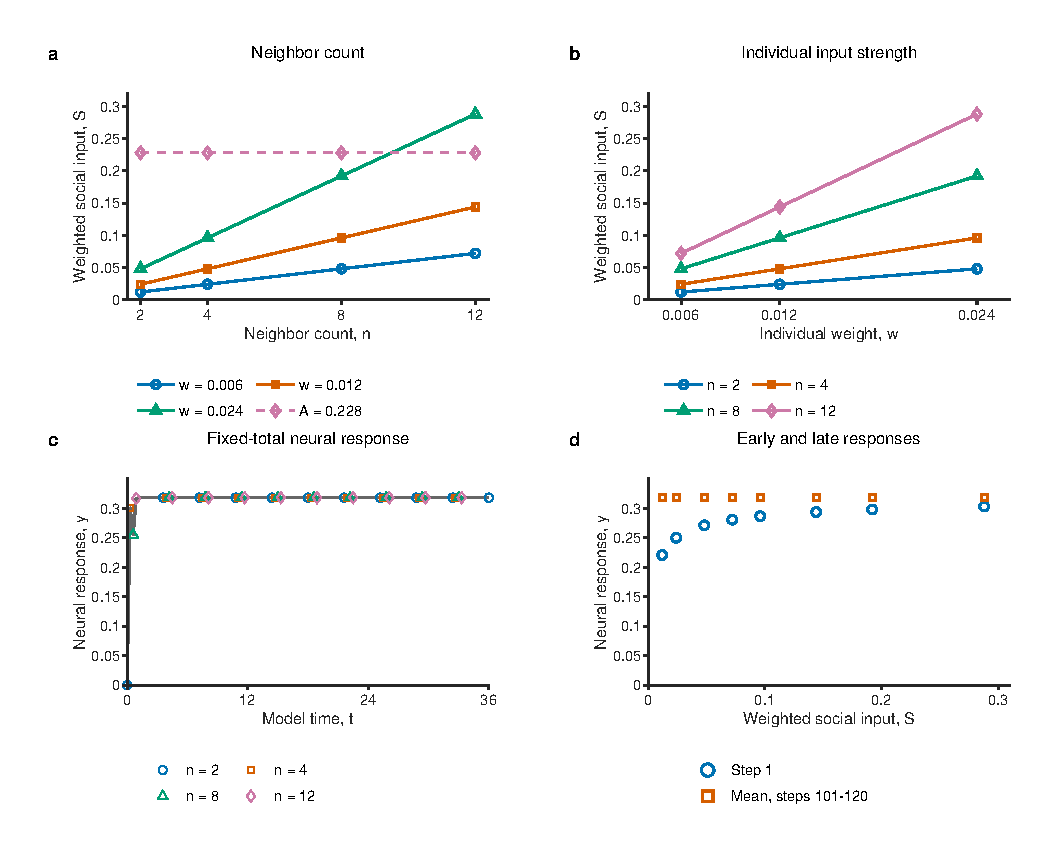
\includegraphics[width=\linewidth]{fig01_count_strength.pdf}
 \caption{正前方输入下的数量与强度累加关系。（a）三种单邻居强度及固定总幅值条件下的 $S_i$--$n_i$ 关系；（b）四种邻居数下的 $S_i$--$w$ 关系；（c）固定 $A_i=0.228$ 时重合的归一化纵向响应，灰线表示共同轨迹，彩色标记在不同时间点采样以便辨识；（d）首步与末 $20$ 步平均响应。纵向响应均除以 $v_sM=5$，时间轴为模型时间。共 $16$ 个确定性条件，$\kappa=1$。}
 \label{fig:exponential_count_strength}
\end{figure}


\subsubsection{实验二：固定总幅值下的方位加权关系}

\textbf{实验条件与基准。} 固定 $n_i=8$、$w=0.0285$、$A_i=0.228$、$\phi_{i,0}=0$。所有邻居取相同方位，从 $-180^\circ$ 到 $165^\circ$、间隔 $15^\circ$ 扫描，共 $24$ 例；另加入前后双峰（各 $4$ 个邻居位于 $0$、$\pi$）、左右双峰（各 $4$ 个位于 $\pm\pi/2$）和圆周均匀（$2\pi j/8$，$j=0,\ldots,7$）三个模板，共 $27$ 例。总幅值基准 $A_i$ 在全部条件下相同，指数模型的解析对照为 $C_i=\exp(\cos\theta-1)$。

\textbf{结果与分析。} 图~\ref{fig:exponential_bearing}a 的重算值与解析曲线一致，正前、正侧和正后方的 $C_i$ 分别为 $1$、$0.3679$ 和 $0.1353$，对应 $S_i=0.2280$、$0.08388$ 和 $0.03086$。三个多峰模板具有不同的完整输入场（图~\ref{fig:exponential_bearing}b），前后双峰、左右双峰和均匀方位结构的 $C_i$ 分别为 $0.5677$、$0.3679$ 和 $0.4658$（图~\ref{fig:exponential_bearing}c）。总幅值保持相同时，方位结构仍能改变加权输入；$C_i$ 因而提供了幅值之外的结构描述。角度扫描的纵向输出随输入方位改变符号（图~\ref{fig:exponential_bearing}d），而指数输入量保持非负。图中标出的对称侧向条件具有数值敏感性，反映了对称输入下的方向解码特征。

\begin{figure}[!tbp]
 \centering
 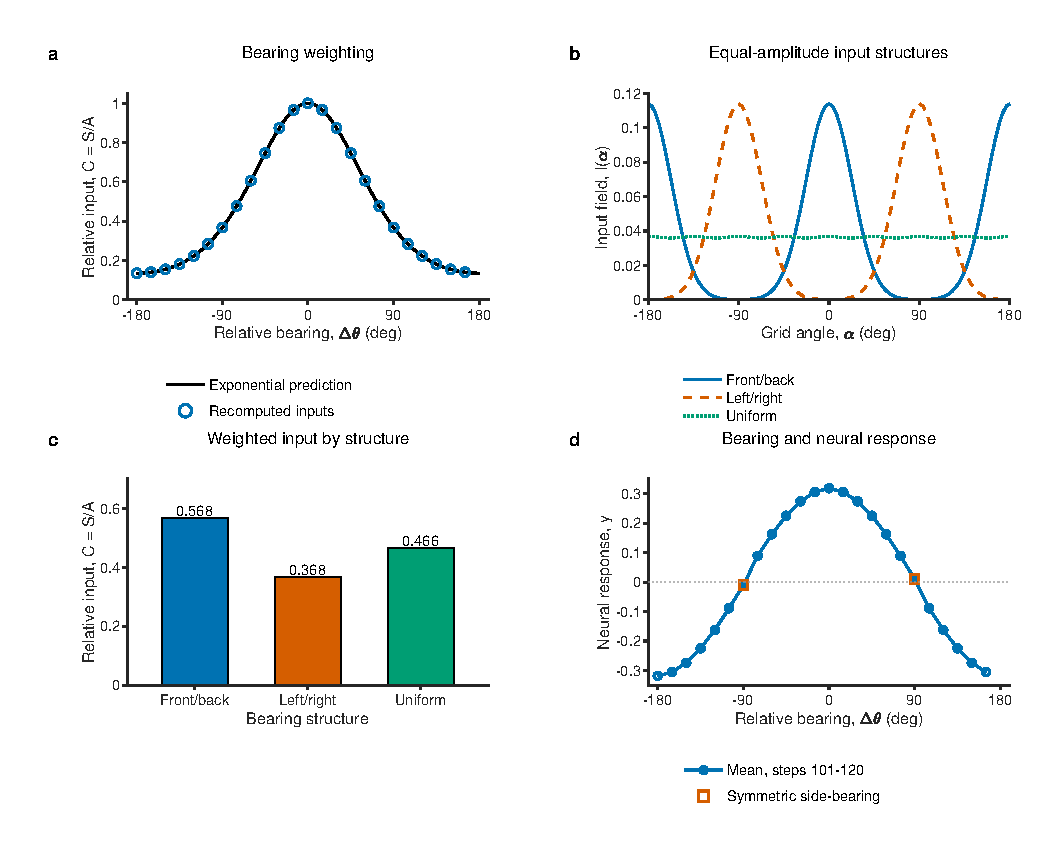
\includegraphics[width=\linewidth]{fig02_bearing_structure.pdf}
 \caption{固定邻居数与总幅值下的方位权重和输入结构。$n_i=8$、$A_i=0.228$、等权输入、$\kappa=1$。（a）间隔 $15^\circ$ 的方位扫描重算值与 $\exp(\cos\Delta\theta-1)$；（b）前后双峰、左右双峰与均匀方位的完整高斯输入场；（c）三个模板的 $C_i=S_i/A_i$；（d）方位扫描的末 $20$ 步平均纵向响应 $y_i$，标记突出 $\pm90^\circ$ 对称侧向条件。角度轴具有周期性。共 $27$ 个条件全部保留；对称侧向输出用于观察数值敏感性。}
 \label{fig:exponential_bearing}
\end{figure}


\subsubsection{实验三：随机输入下的神经场响应对照}

\textbf{实验条件。} 取 $n_i\in\{2,4,8,12\}$、$A_i\in\{0.114,0.228,0.456\}$ 和 $20$ 组随机几何输入，共 $240$ 例。每组使用 MATLAB 的 \texttt{mt19937ar} 随机流，种子为 $20261011$--$20261030$，按顺序生成 $12$ 个 $\mathrm{Uniform}(-\pi,\pi)$ 方位、$12$ 个 $\mathrm{Uniform}(0.5,1.5)$ 原始权重和 $1$ 个 $\mathrm{Uniform}(-\pi,\pi)$ 初始自身朝向。各邻居数取前 $n_i$ 个目标，将权重归一化到给定 $A_i$；同一种子的 $12$ 个条件共用方位、原始权重和初始朝向。

\textbf{基准与统计方法。} 分别以 $X_i=A_i$ 和 $X_i=S_i$ 建立带截距的一元线性回归 $Y_i=a+bX_i$，采用按几何种子分组的留一组交叉验证。每轮整体留出同一种子的 $12$ 例测试，其余 $228$ 例训练，$\kappa=1$ 固定。以全部留出预测的归一化 RMSE 衡量响应预测误差，以每个几何种子的归一化 MSE 作配对比较。使用 $5000$ 次成对几何组 bootstrap，报告百分位 $95\%$ 区间，随机流为 NumPy PCG64、种子 $2026101101$；重采样单位为 $20$ 个几何组，区间基于已拟合的留出误差，未在各次 bootstrap 内重新拟合。描述性的分层相关采用预先固定的方向判据：解码方向向量模大于 $10^{-9}$ 时方向有效，否则将该步运动向量记为零。

\textbf{结果与分析。} 图~\ref{fig:exponential_random_response}a 显示，相同总幅值下仍存在不同的输入加权量与纵向响应。加入方位权重后，归一化测试 RMSE 从幅值基准的 $0.2060$ 降至 $0.1729$，相对降低 $16.1\%$（图~\ref{fig:exponential_random_response}b、d；表~\ref{tab:exponential_response}）。$20$ 个几何组中有 $18$ 个的测试 MSE 更低（图~\ref{fig:exponential_random_response}c）。配对归一化 MSE 降低量 $\mathrm{MSE}_A-\mathrm{MSE}_S$ 的均值为 $0.01257$，$95\%$ bootstrap 区间为 $[0.00835,\,0.01687]$。在具有响应变化的 $10$ 个 $(n_i,A_i)$ 分层中，$S_i$ 与 $y_i$ 的 Spearman 相关系数为 $0.599$--$0.920$；另外两个低幅值分层的输出为零，相关系数未定义。该结果支持相对总幅值基准的局部预测关联；尚未比较加权余弦投影、圆周合矢量或低阶 Fourier 描述，也未验证时变群体 GO、LO 与凝聚响应。交叉验证训练集互相重叠，当前区间仅对已得到的留出误差作组重采样，不涵盖重新选模型或重新拟合的全部不确定性。

\begin{table}[!tbp]
 \centering
 \caption{随机几何分组交叉验证的归一化响应误差。两种模型使用相同的单变量线性回归及分组划分，共 $20$ 个几何组、$240$ 个配对条件。区间由几何组 bootstrap 得到。}
 \label{tab:exponential_response}
 \begin{tabular}{lcc}
  \toprule
  模型输入 & 测试 RMSE & $95\%$ bootstrap 区间\\
  \midrule
  总幅值 $A_i$ & $0.2060$ & $[0.1789,\,0.2319]$\\
  指数加权输入 $S_i$ & $0.1729$ & $[0.1515,\,0.1937]$\\
  \bottomrule
 \end{tabular}
\end{table}

\begin{figure}[!tbp]
 \centering
 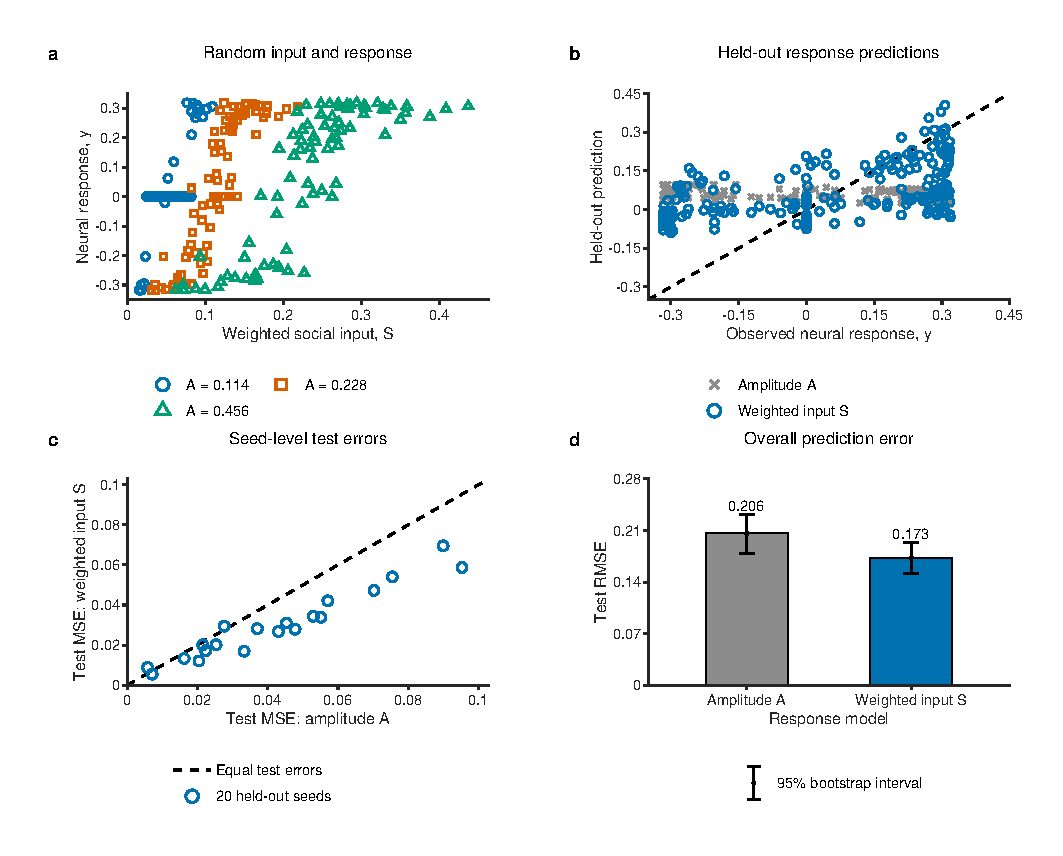
\includegraphics[width=\linewidth]{fig03_random_response.pdf}
 \caption{随机几何输入下的留出响应预测。$20$ 组几何各含 $12$ 个数量--幅值条件，共 $240$ 例。（a）$S_i$ 与归一化响应 $y_i=Y_i/5$，按总幅值分组；（b）总幅值模型和指数加权模型的留出预测，虚线为预测与观测相等；（c）各几何组的测试 MSE，虚线下方表示指数加权模型误差较小，共 $18/20$ 组；（d）全部留出预测的 RMSE。每折整体留出一个几何种子；误差棒为对已拟合留出误差进行 $5000$ 次配对几何组 bootstrap 的 $95\%$ 百分位区间。}
 \label{fig:exponential_random_response}
\end{figure}


\subsection{社会输入机制的基准影响}

图~\ref{fig:input_mechanism} 同时给出输入幅值、角度覆盖、输入集中度、GO、LO 和凝聚距离。随机选邻并采用模型原定单邻居幅值时，增加 $n_e$ 会同时提高输入幅值和方向采样密度，使 GO、LO 上升并减小凝聚距离。固定总幅值后，输入幅值基本保持不变，但角度覆盖和输入集中度仍随选邻策略变化，反映了方向采样的作用。该结果支持将输入幅值和方位结构作为两个相互耦合且可区分的因素，并分别评价其对群体运动的影响。

\begin{figure}[!tbp]
 \centering
 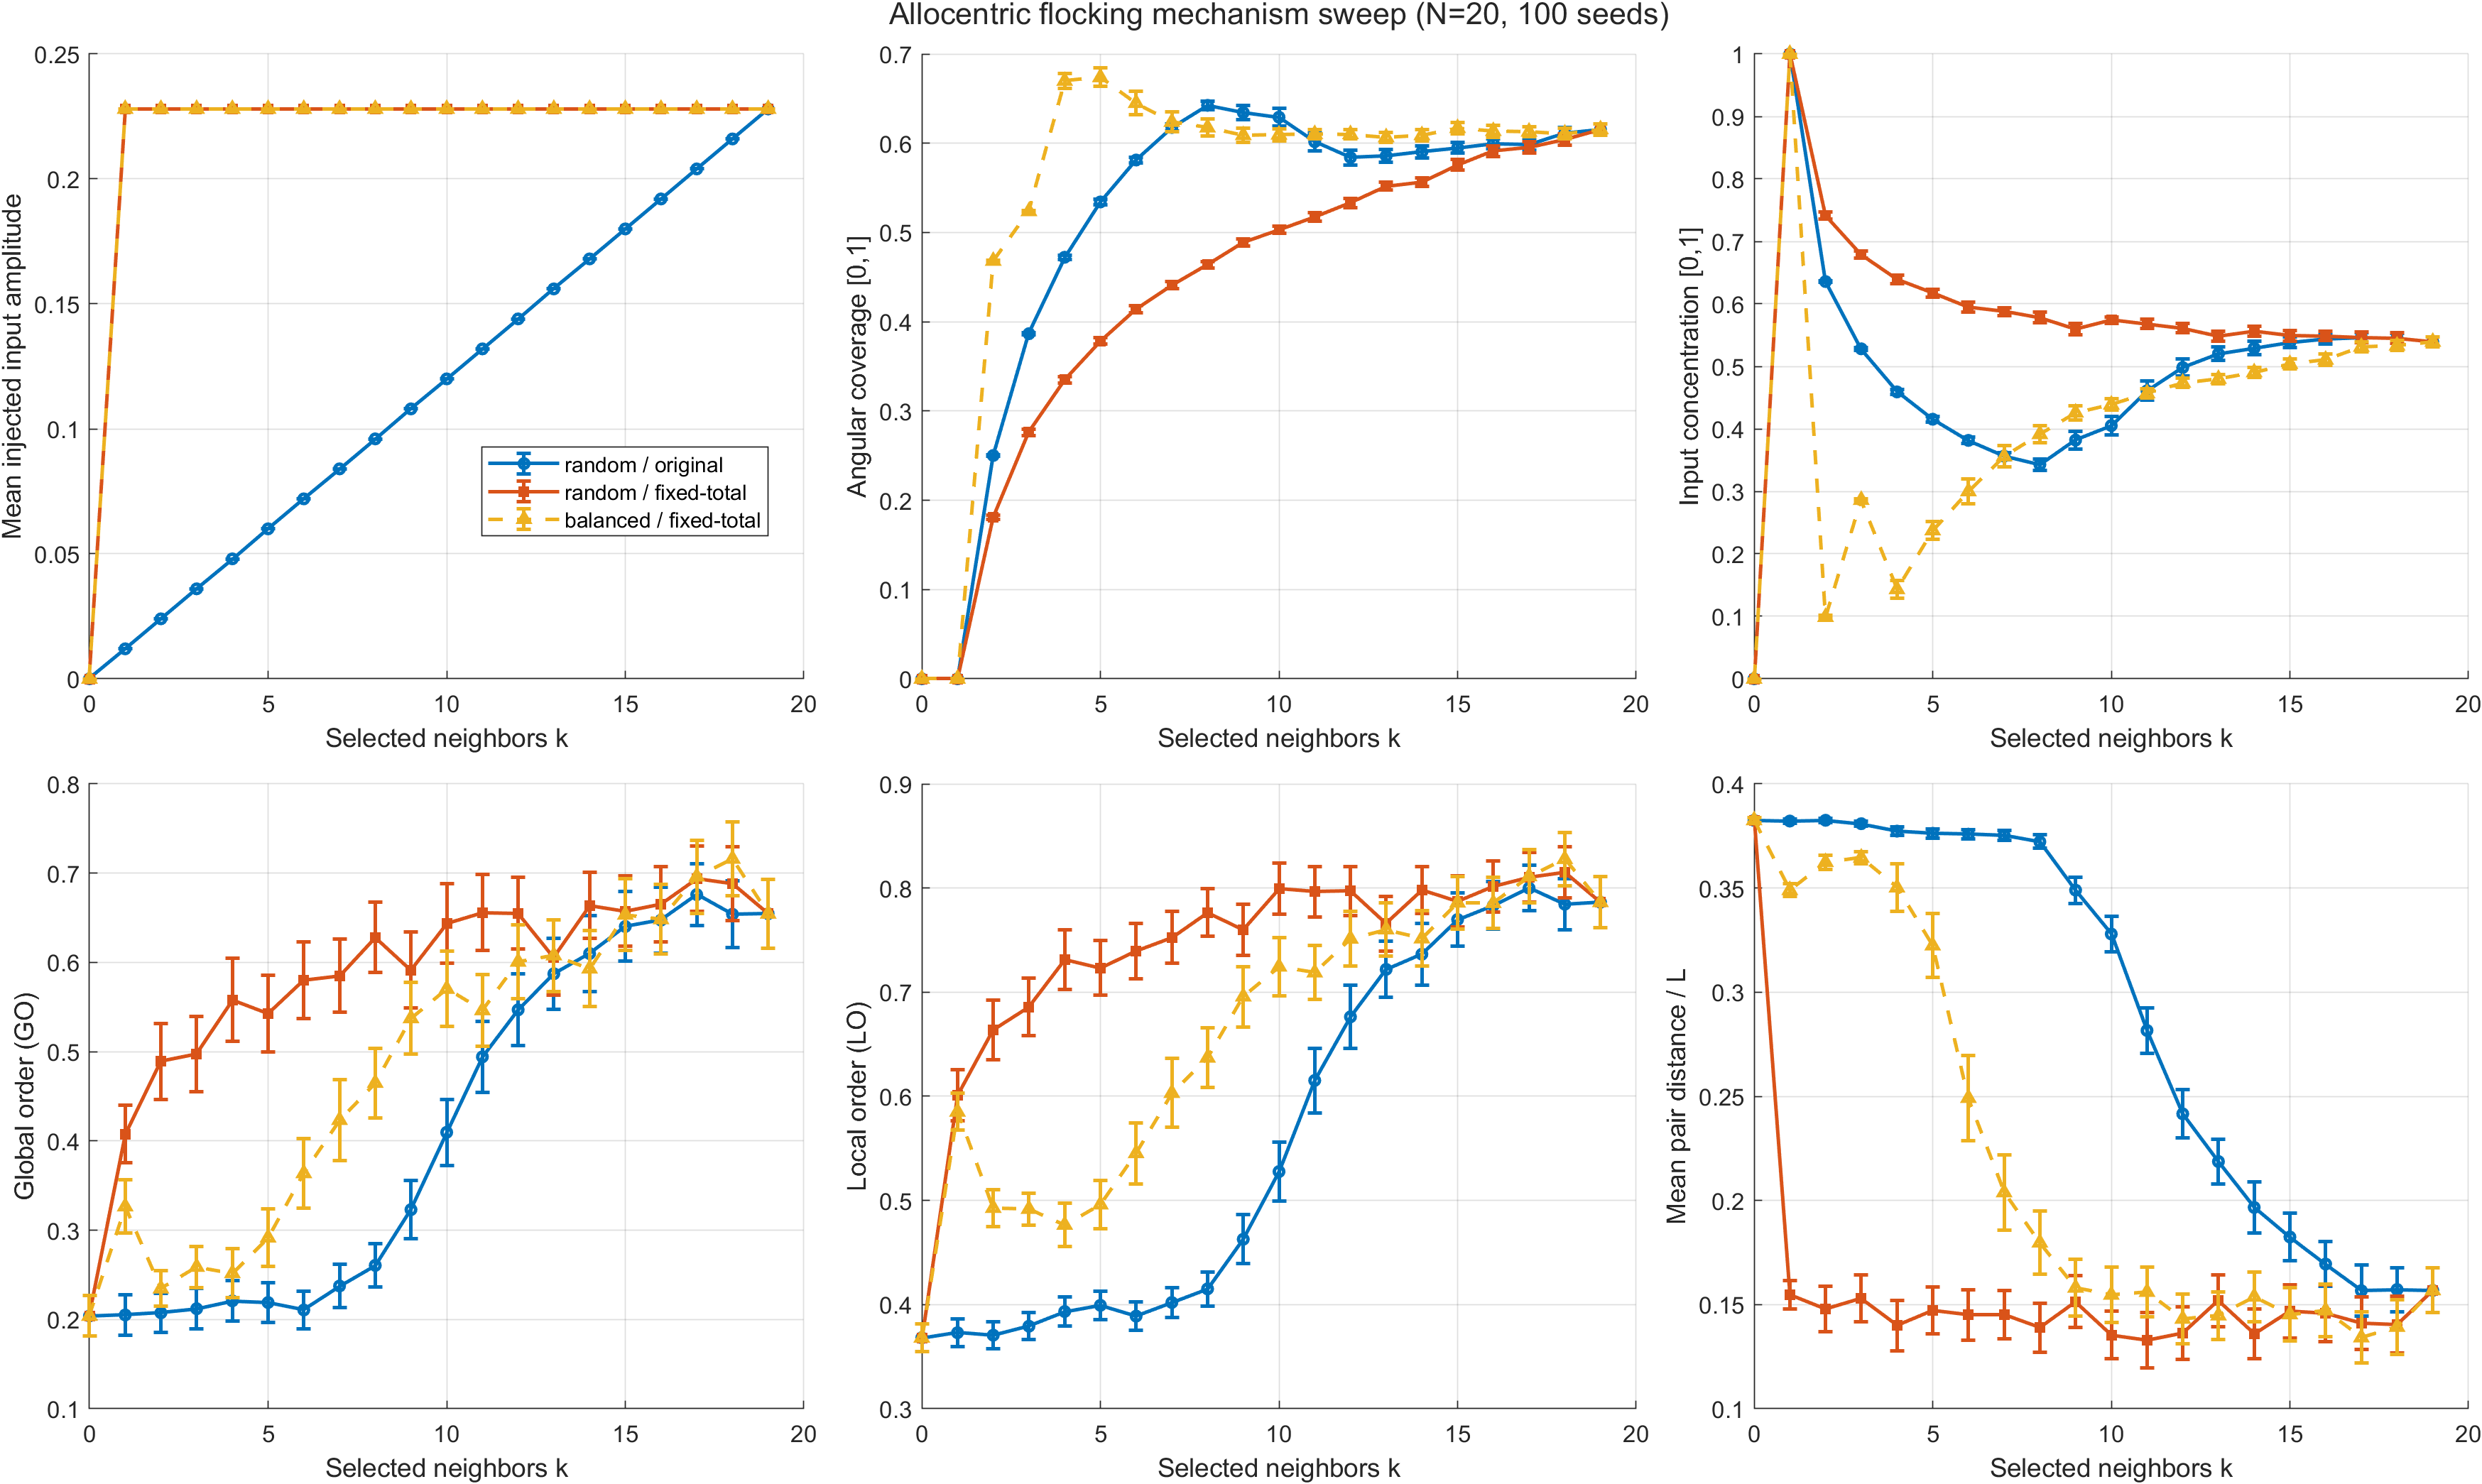
\includegraphics[width=0.96\linewidth]{fig1_input_mechanism.png}
 \caption{邻居数量、输入幅值和方位选择策略的机制分解（N=20，种子 1--100）。}
 \label{fig:input_mechanism}
\end{figure}

\subsection{连续缺失下的协方差与方位预测}

连续缺失期间，常角速度模型的方位方差满足
\begin{equation}
 V(T)=p_{11}+2Tp_{12}+T^2p_{22}+q_\omega T^3/3
\end{equation}
其中短期单调性还取决于交叉协方差。周期卷积对第 $n$ 阶方向谐波的衰减为 $\exp(-n^2V/2)$，随缺失时间增加展宽方向核并抑制高阶方向结构，同时保留总输入。图~\ref{fig:uncertainty_diagnostics} 的上排给出该解析性质，下排给出离线预测误差和 95\% 经验覆盖率。较长遮挡下的覆盖率明显低于名义值，表明协方差低估了实际误差，后续需要按经验覆盖率校准。卷积会展宽方向核，但当前结果尚不能把闭环差异唯一归因于展宽：方差门控也会改变激活边集合。

\begin{figure}[!tbp]
 \centering
 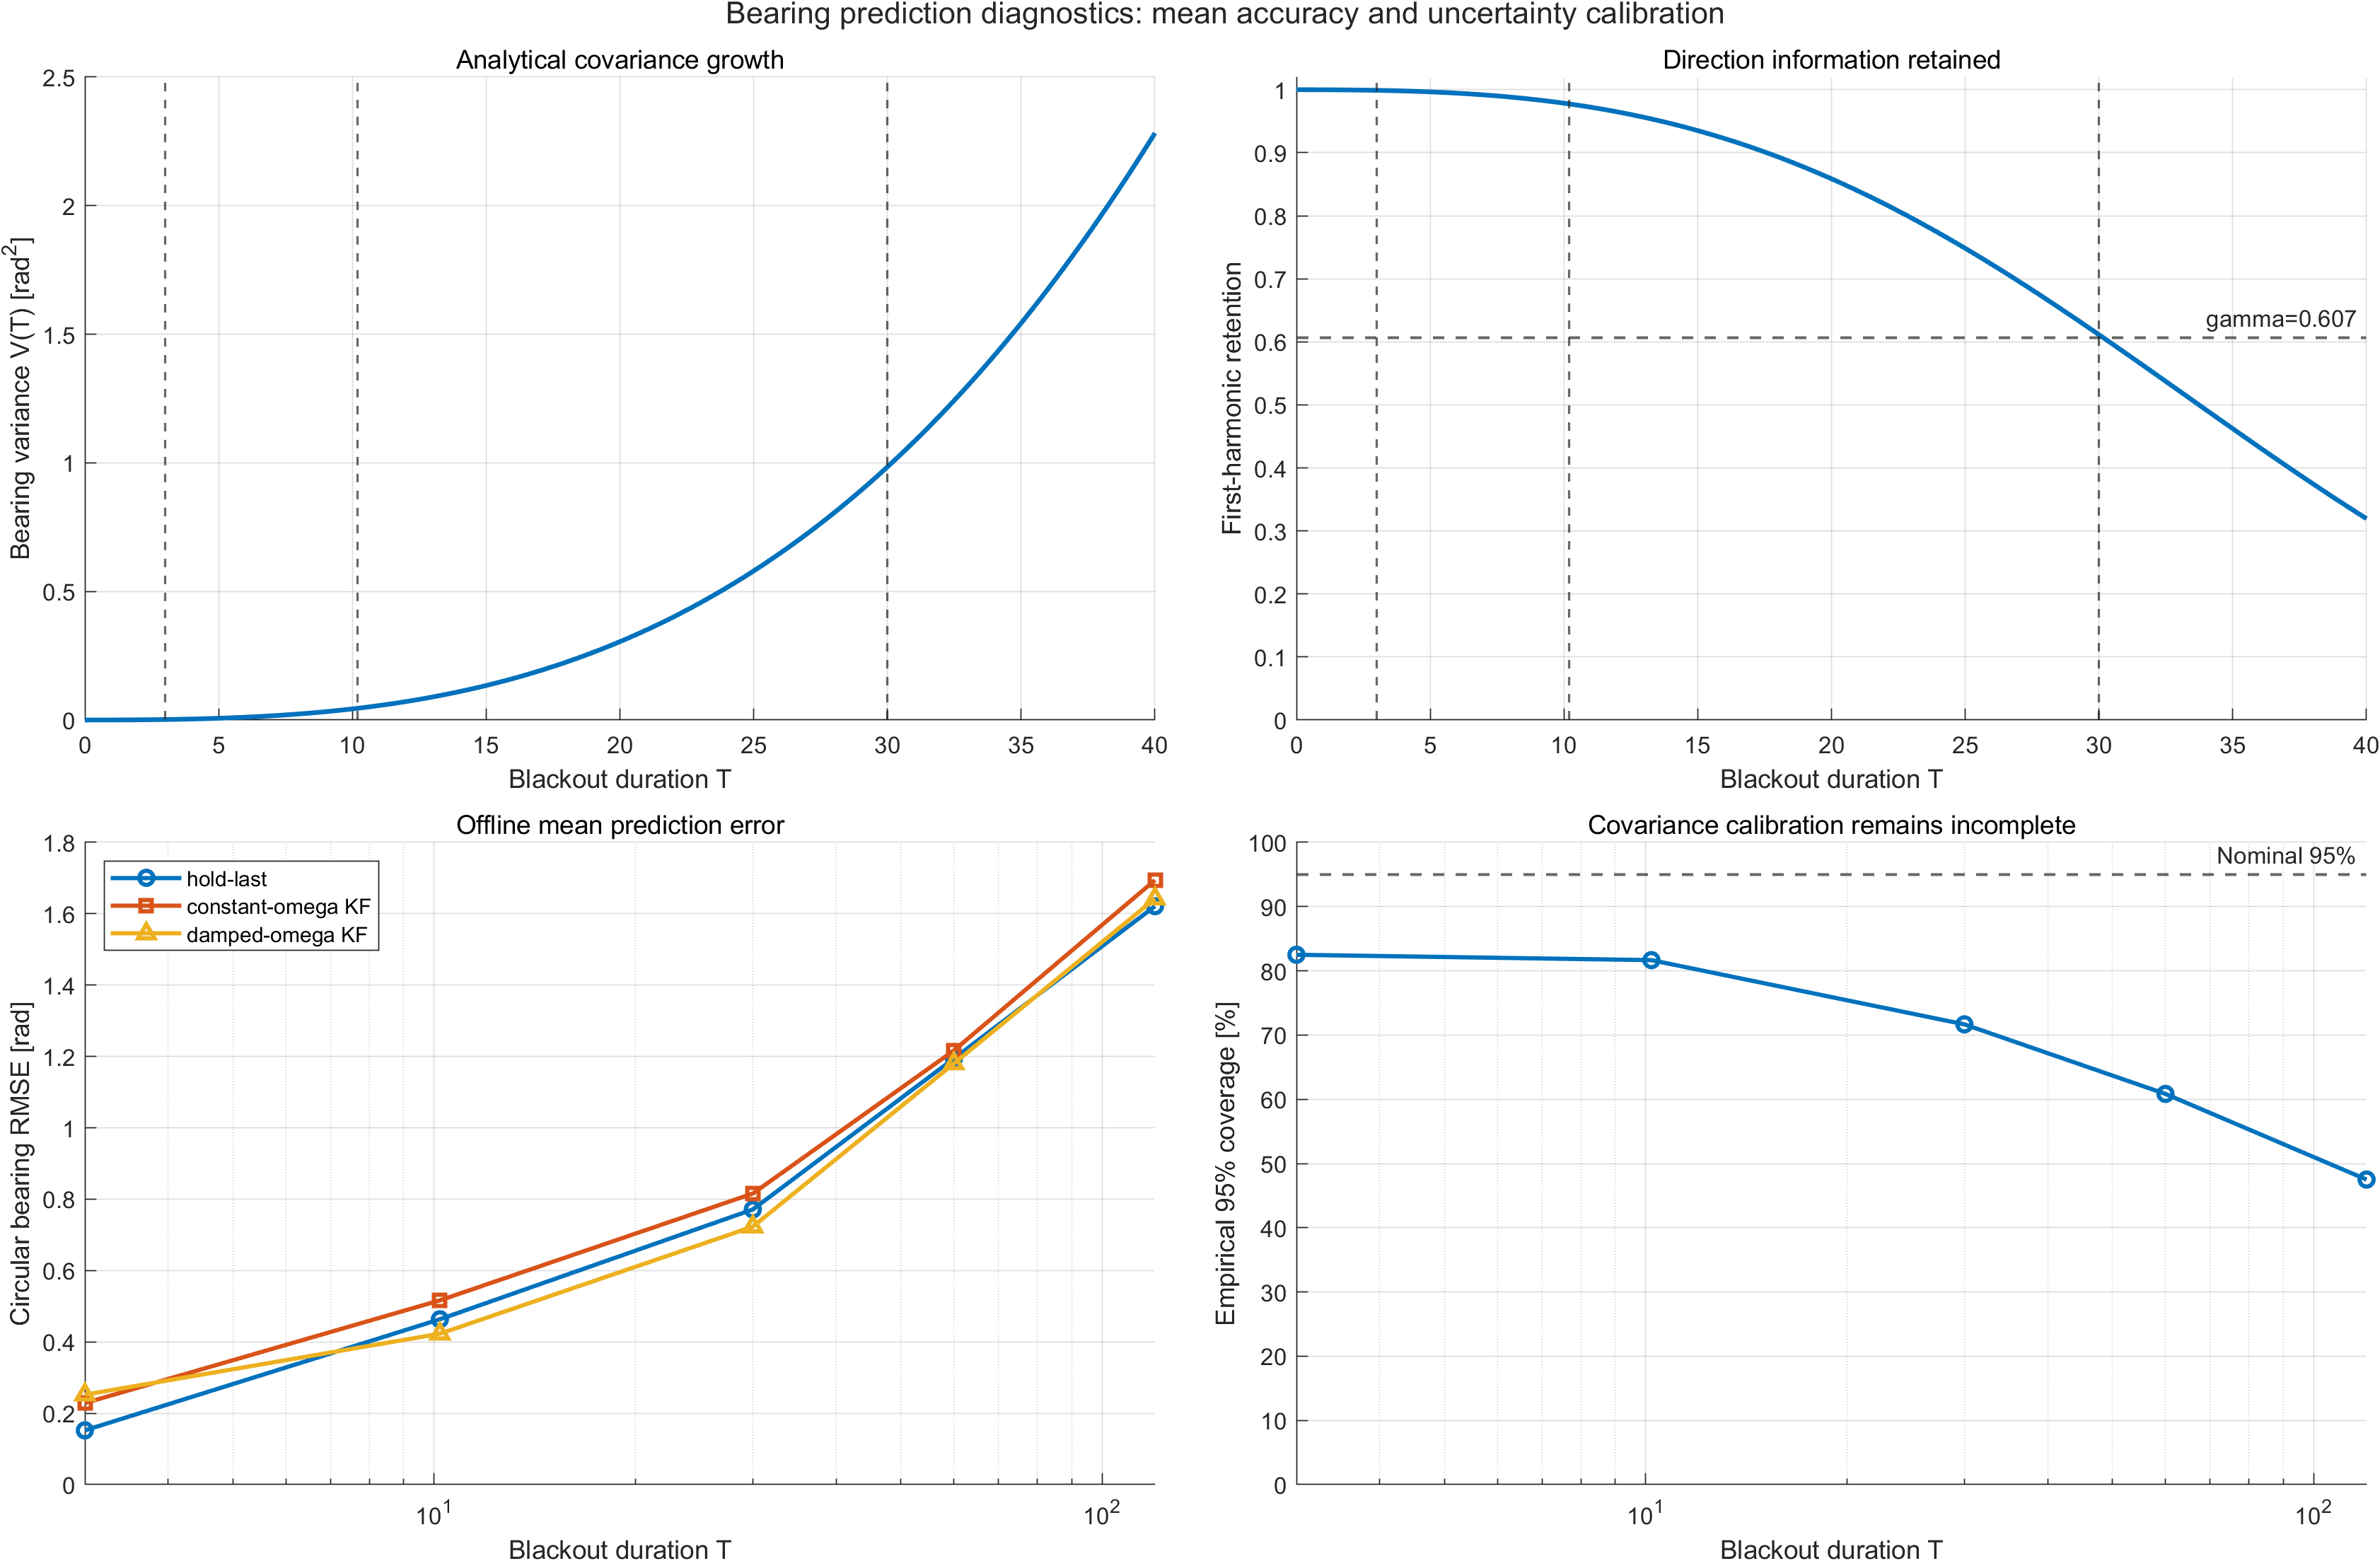
\includegraphics[width=0.98\linewidth]{kf-uncertainty-diagnostics.png}
 \caption{方位预测诊断。上排为解析协方差与方向信息保持；下排为离线均值误差和 95\% 经验覆盖率（种子 138--141）。}
 \label{fig:uncertainty_diagnostics}
\end{figure}

图~\ref{fig:predict_error} 进一步给出隐藏边上的平均方位预测误差。相较 hold-last，阻尼角速度 KF-GM-uncertainty 在 $6\le T\le30$ 时将预测误差降低约 $13\%$--$19\%$，配对 bootstrap 区间不跨零；在 $T=60$ 时仍降低约 $9\%$--$10\%$。$T=3$ 时均值降低约 $11\%$--$13\%$，但在两种较强遮挡条件下区间略跨零，因此只视为方向一致的短期改善。需区分误差评价的有效窗口：扩展批次仅在缺失且仍激活的边上累计预测误差。$T=60$ 共 $200$ 步，常角速度 KF 在方差门限作用下仅纳入前 $100$ 步，而 hold 和 GM 纳入全部 $200$ 步。例如隐藏 $11$ 边时，每种子的计数分别为 $22000$ 与 $44000$。因此本稿不将常角速度 KF 在 $T=60$ 的较小误差解释为完整窗口预测优势，并在图中省略该不可比点。闭环 GO 与距离仍按完整窗口计算，描述的是预测与门控的组合效果。

\begin{figure}[!tbp]
 \centering
 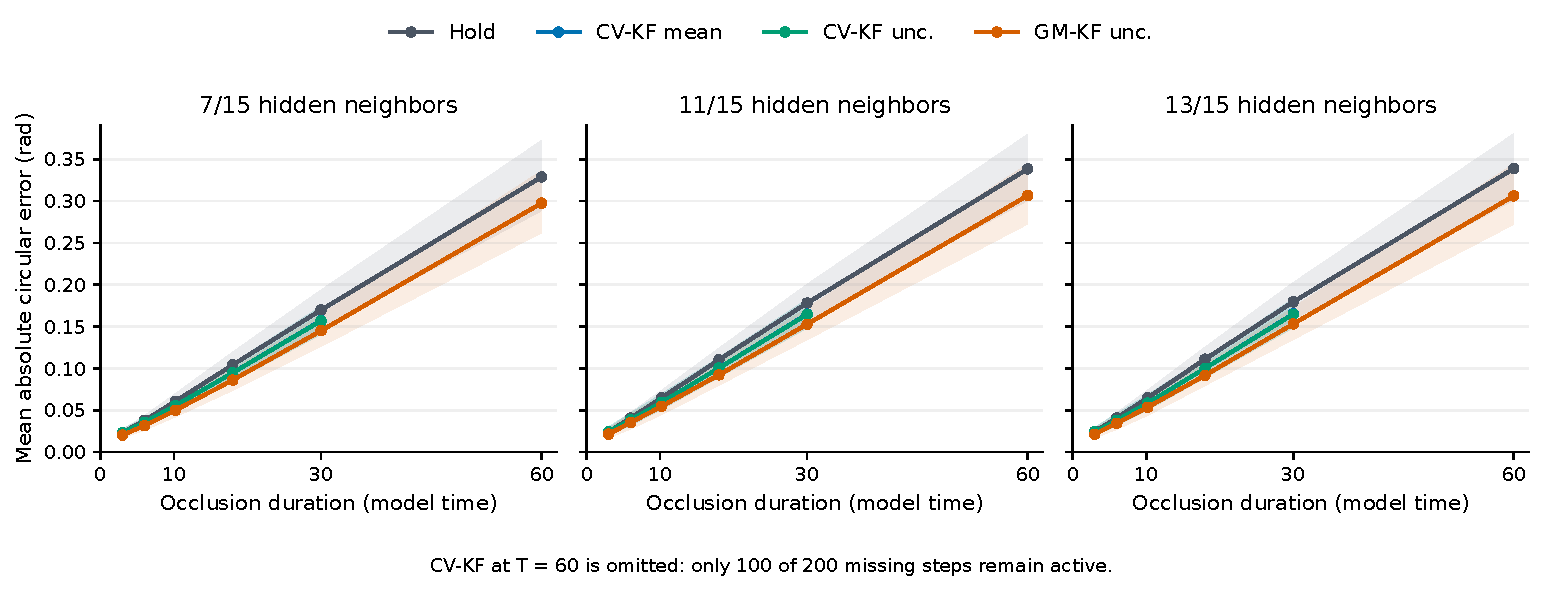
\includegraphics[width=\linewidth]{kf-prediction-error-v4.pdf}
 \caption{扩展批次隐藏且激活边的平均绝对圆周误差，$30$ 个种子；阴影为种子配对 bootstrap 的逐条件 $95\%$ 区间。常角速度 KF 在 $T=60$ 的有效窗口只有半程，故不展示该点。该指标不是五种子批次的 RMSE；真值仅用于诊断。}
 \label{fig:predict_error}
\end{figure}


\subsection{方位预测与输入重建的分层机制实验}
\label{sec:kf_pilot}

本节以离线方位预测、同状态输入重建和检查点分叉闭环三个层次，检验历史方位预测如何转化为神经场输入，并观察输入变化对应的群体运动响应。采用五个开发种子 $1$--$5$，以逐种子配对结果描述不同补偿策略的作用。

\subsubsection{实验条件与对照方法}

每个智能体固定选择编号向后的 $8$ 个循环邻居，等权输入，总权重记为 $A_0$。完整观测运行至第 $6200$ 步，在最后合法观测上冻结隐藏邻居身份；第 $6201$--$6234$ 步屏蔽方位，共 $34$ 步，即 $10.2$ 个模型时间单位，第 $6235$ 步恢复，仿真运行至第 $6600$ 步。观测无噪声，方位采用世界坐标系，输入强度保持最后合法值。KF 采用常角速度状态，$q_\omega=10^{-6}$、$R=10^{-4}$、$P_0=\operatorname{diag}(R,1)$，初始角速度为零。此处 $R$ 为固定的假定观测方差与数值正则量；协方差通过覆盖率和恢复首步 NIS 诊断。

围绕中心条件 $h=4$、random、$A_0=0.228$，分别扫描隐藏邻居数 $h\in\{2,4,6\}$、隐藏方位结构 random/concentrated/dispersed，以及 $A_0\in\{0.114,0.228,0.456\}$，共 $7$ 个唯一条件。concentrated 和 dispersed 在最后合法观测上分别选择一阶圆周合矢量模 $R_1^{\mathcal H}=|h^{-1}\sum_{j\in\mathcal H_i}e^{\mathrm{i}\theta_{ij}}|$ 最大和最小的隐藏集合。每个 $A_0$ 均重新运行完整前缀，同一 $(\text{seed},A_0)$ 内各方法共享检查点；幅值扫描因而同时包含预热动力学的变化。

对照包括：fresh 始终使用完整当前观测；drop 删除缺失边；drop-normalized 将可见边权重调整为 $A_0/(8-h)$，保持总幅值；hold 保持缺失边的最后方位及权重；KF-mean 按式~\eqref{eq:pilot_causal_input} 注入预测均值。drop 对应幅值与方位同时减少，drop-normalized 保留幅值而减少方位覆盖，hold 延续历史方位，KF-mean 在相同缓存权重上增加方向外推。恢复首步各方法均使用当前合法观测。新批次评估均值外推及协方差诊断，协方差卷积的闭环结果在后续扩展时长实验中分别报告。

每个种子有 $3$ 条 fresh 参考轨迹和 $7\times4=28$ 条非 fresh 轨迹，五个种子共 $155$ 条唯一闭环轨迹；同一 fresh 轨迹在对应条件中重复引用。另有 $35$ 组同状态输入回放，以及 $7\times5\times3=105$ 项离线 $R$ 诊断，其中替代 $R=10^{-6},10^{-2}$ 均使用相同的完整 $6200$ 步合法历史。统计按种子配对，采用 $5000$ 次种子组 bootstrap，随机种子为 $20261010$，所有条件共用重采样索引。

\subsubsection{评价指标与解释}

离线层在 fresh 轨迹上屏蔽固定邻居观测，以缺失期间全部隐藏边--时间点的圆周误差计算每个种子的方位 RMSE，再对五个种子取均值。覆盖率为 $|e_{ij}|\le1.96\sqrt{P_{11,ij}^{-}}$ 的边--时间点比例；归一化创新平方（NIS）为恢复首步的 $\nu_{ij}^2/(P_{11,ij}^{-}+R)$，在隐藏边上取均值，用于比较预测创新与假定方差。同状态层让各候选输入读取相同 fresh 状态，比较完整神经场输入向量，定义
\begin{equation}
 E_I^{(s)}=\frac{1}{N|\mathcal K_o|}
 \sum_{k\in\mathcal K_o}\sum_{i=1}^N
 \frac{\|I_i^{(s)}(k)-I_i^{\mathrm{fresh}}(k)\|_2}
 {\|I_i^{\mathrm{fresh}}(k)\|_2}.
 \label{eq:pilot_input_error}
\end{equation}
该误差直接描述在相同几何状态下输入场的重建程度；第~\ref{sec:social_input_model} 节的 $S_i$ 则描述方位加权后的标量输入量。

闭环层在共同检查点上分别推进，主响应为恢复后 $100$ 步，即 $\mathcal K_r=\{6235,\ldots,6334\}$ 内的有符号平均对距变化
\begin{equation}
 \Delta D^{(s)}=\frac{1}{|\mathcal K_r|}\sum_{k\in\mathcal K_r}
 \frac{d^{(s)}(k)-d^{\mathrm{fresh}}(k)}{L},
 \quad
 D_{\mathrm{abs}}^{(s)}=\frac{1}{|\mathcal K_r|}\sum_{k\in\mathcal K_r}
 \frac{|d^{(s)}(k)-d^{\mathrm{fresh}}(k)|}{L},
 \label{eq:pilot_distance_metrics}
\end{equation}
其中 $d$ 为周期最短两两距离均值。$\Delta D$ 的正、负值分别表示相对 fresh 更分散、更紧凑，$D_{\mathrm{abs}}$ 补充描述偏离大小。GO 和 LO 的损失定义为相同窗口内 fresh 减去候选分支的时间平均值。

\subsubsection{方位预测及协方差诊断结果}

中心条件下，KF-mean 的逐种子 RMSE 均值为 $0.1040$ rad，hold 为 $0.1414$ rad，降低 $26.4\%$，五个种子中四个误差更低。种子 $2$ 的 KF 误差为 $0.3757$ rad，高于 hold 的 $0.2348$ rad，体现了常角速度外推对具体轨迹的敏感性。图~\ref{fig:kf_pilot_prediction}a--c 中，隐藏数量从 $2$ 增至 $6$ 时，KF 均值误差从 $0.1012$ 增至 $0.1148$ rad；集中与分散结构下分别为 $0.0976$ 和 $0.1396$ rad。低幅值 $A_0=0.114$ 时 KF 为 $0.2229$ rad，高于 hold 的 $0.2002$ rad；$A_0=0.456$ 时 KF 降至 $0.000481$ rad。这些变化反映了不同输入条件及其预热轨迹下的预测表现。

\paragraph{汇总方式与小样本敏感性}
中心条件各个种子均有 $2720=20\times4\times34$ 个隐藏边--时间点。设第 $r$ 个种子的 RMSE 为 $r_r$，则逐种子平均为 $5^{-1}\sum r_r$，合并平方误差后的 RMSE 为 $\sqrt{5^{-1}\sum r_r^2}$。两种估计量回答不同问题，统计重采样单位均为种子。表~\ref{tab:rmse_sensitivity} 保留全部五个种子：KF 在 $4/5$ 个种子改善，但种子 $2$ 的大误差使合并 RMSE 比 hold 增高 $13.5\%$。逐种子 RMSE 差值（KF 减 hold）为 $-0.03739$ rad，配对种子 bootstrap 的 $95\%$ 区间为 $[-0.11198,0.06002]$，跨零。因此 $26.4\%$ 不能概括为稳定或统计上已确认的方位预测收益。

\begin{table}[!tbp]
\centering\small
\caption{中心条件方位 RMSE 的逐种子值与汇总敏感性（rad）。全部记录保留，未排除大误差种子。}
\label{tab:rmse_sensitivity}
\begin{tabular}{lrr}
\toprule 种子或汇总方式 & hold & KF-mean\\\midrule
1 & 0.150014 & 0.000677\\
2 & 0.234778 & 0.375660\\
3 & 0.095930 & 0.039982\\
4 & 0.162777 & 0.091770\\
5 & 0.063641 & 0.012095\\\midrule
逐种子 RMSE 均值 & 0.141428 & 0.104037\\
合并平方误差后开根号 & 0.153215 & 0.173947\\\bottomrule
\end{tabular}
\end{table}

主 $R$ 下，中心条件的名义 $95\%$ 区间经验覆盖率为 $89.76\%$，种子范围为 $65.74\%$--$100\%$，恢复首步平均 NIS 为 $76.45$。图~\ref{fig:kf_pilot_prediction}d 显示不同假定 $R$ 下覆盖率的种子差异，种子 $2$ 的低覆盖率与其较大预测误差相对应。由此，预测均值改善与协方差校准需要分别评价，后续将以经验覆盖率校准不确定性传播。

\begin{figure}[!tbp]
 \centering
 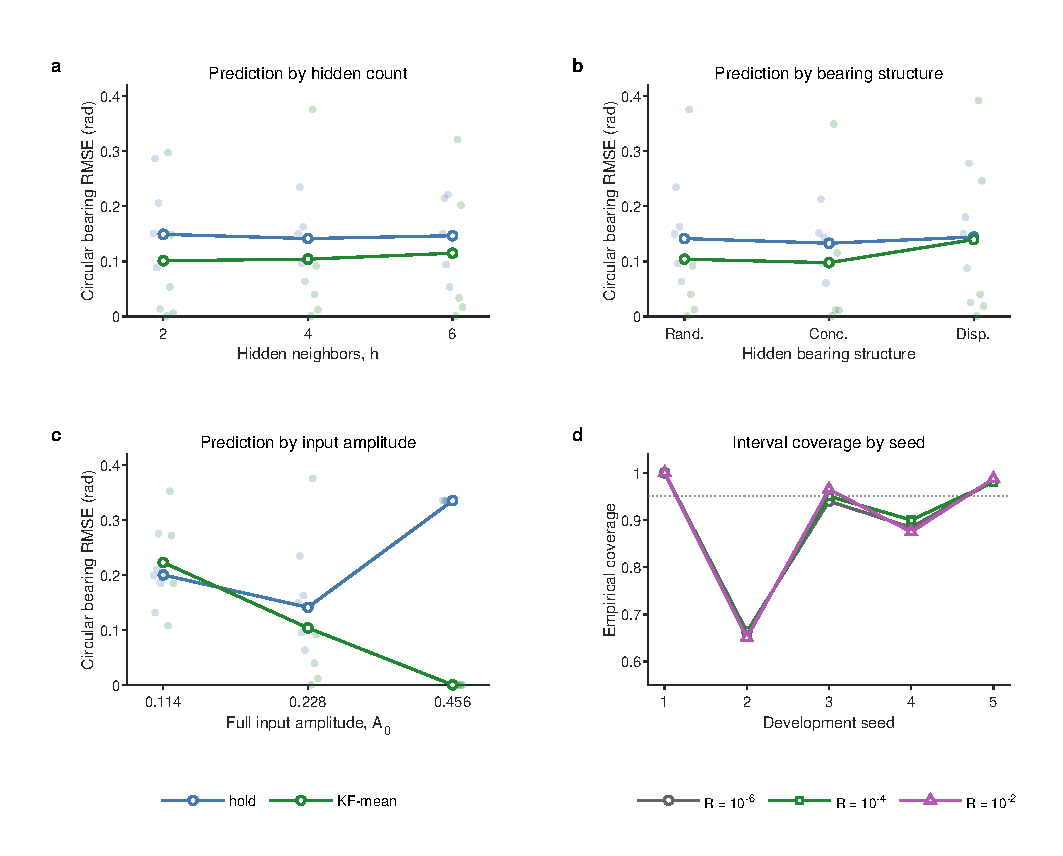
\includegraphics[width=\linewidth]{fig04_kf_prediction.pdf}
 \caption{五种子开发实验中的方位预测与覆盖率诊断。（a--c）分别扫描隐藏邻居数、隐藏方位结构和完整观测总幅值；连线点为五个逐种子圆周 RMSE 的均值，浅色散点为各种子值，主 $R=10^{-4}$。三个扫描共享中心条件 $h=4$、random、$A_0=0.228$。（d）中心条件下三个假定 $R$ 的逐种子经验覆盖率，虚线为名义 $0.95$。全部条件的连续缺失时长为 $34$ 步、$10.2$ 个模型时间单位；重采样单位为 $5$ 个开发种子。}
 \label{fig:kf_pilot_prediction}
\end{figure}


\subsubsection{同状态输入重建与闭环响应}

表~\ref{tab:kf_pilot_center} 中，中心条件的同状态输入误差从 drop 的 $0.5143$ 降至 drop-normalized 的 $0.2671$，说明恢复总幅值能够补偿部分输入差异。hold 进一步降至 $0.05507$，KF-mean 降至 $0.02103$，相对 hold 降低 $61.8\%$。按种子配对的误差差值（KF 减 hold）为 $-0.03404$，$95\%$ bootstrap 区间为 $[-0.06738,-0.00790]$，仅反映这五个开发种子的有限证据。二者使用相同的缓存权重，差异来自缺失期间的方向外推，表明预测方位能够在保持历史输入的基础上进一步重建当前方向场。

\begin{table}[!tbp]
 \centering
 \small
 \caption{中心条件下五个种子的平均响应。$h=4$、random、$A_0=0.228$；输入误差在同一 fresh 状态上计算，距离与 GO 在闭环恢复后 $100$ 步计算。距离列及 GO 损失列按表头缩放；$\Delta D$ 为有符号变化，$D_{\mathrm{abs}}$ 为逐时刻绝对偏离的平均值。}
 \label{tab:kf_pilot_center}
 \begin{tabular}{lrrrr}
  \toprule
  方法 & $E_I$ & $10^3\Delta D$ & $10^3D_{\mathrm{abs}}$ & $10^3$ GO 损失\\
  \midrule
  fresh & $0$ & $0$ & $0$ & $0$\\
  drop & $0.51426$ & $1.60580$ & $1.60580$ & $-7.09418$\\
  drop-normalized & $0.26710$ & $0.07157$ & $0.32839$ & $-2.16612$\\
  hold & $0.05507$ & $0.58979$ & $0.58979$ & $-1.86953$\\
  KF-mean & $0.02103$ & $0.08120$ & $0.08181$ & $-1.34723$\\
  \bottomrule
 \end{tabular}
\end{table}

闭环层的响应体现了输入重建与群体指标之间的非线性联系。中心条件下，KF-mean 的 $\Delta D=8.12\times10^{-5}$，hold 为 $5.90\times10^{-4}$；drop-normalized 的有符号均值略低于 KF，但其绝对偏离为 $3.28\times10^{-4}$，高于 KF 的 $8.18\times10^{-5}$，说明符号抵消会影响单纯均值比较。四种非 fresh 分支的中心条件 GO 损失均为负，即该窗口内 GO 略高于 fresh，同时仍存在距离结构偏移，体现了有序度与凝聚响应的不同侧面。

图~\ref{fig:kf_pilot_input_response}a--c 显示，增加隐藏数量使输入场重建误差上升；在七个条件中 KF-mean 的平均输入误差均低于 hold。图~\ref{fig:kf_pilot_input_response}d--f 的对距变化则具有非单调性：数量扫描中 KF 的有符号变化为 $6.51\times10^{-5}$、$8.12\times10^{-5}$、$2.74\times10^{-5}$；分散结构及高幅值条件的均值略为负。在 $35$ 个种子--条件配对中，KF 相对 hold 的有符号变化和绝对偏离分别在 $34$ 项中更低，各项共享同一批五个种子。结果支持将方位预测、输入场重建和闭环响应逐层评价：预测提供的方向信息改善了输入重建，群体指标还受神经场非线性与分叉轨迹影响。

\begin{figure}[!tbp]
 \centering
 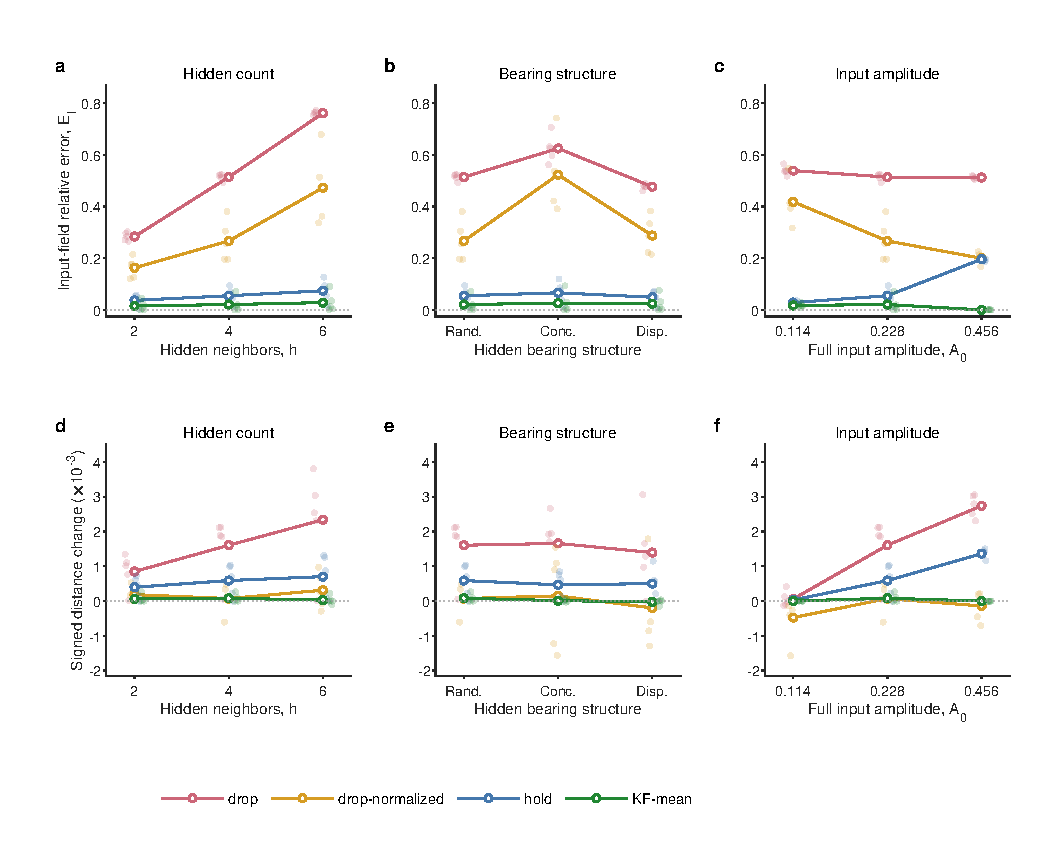
\includegraphics[width=\linewidth]{fig05_kf_input_response.pdf}
 \caption{输入重建与闭环对距响应的三条单因素扫描。（a--c）缺失期间在同一 fresh 状态上计算的完整输入场相对误差 $E_I$；（d--f）恢复后 $100$ 步的有符号对距变化 $\Delta D$，纵轴单位为 $10^{-3}$。各列分别改变隐藏数量、方位结构和完整观测总幅值，中心条件与图~\ref{fig:kf_pilot_prediction} 一致。连线点为五种子均值，浅色散点为逐种子值；零线对应 fresh 参考。负值表示相对 fresh 更紧凑，连线用于辨识三个离散水平。}
 \label{fig:kf_pilot_input_response}
\end{figure}


\subsection{扩展遮挡时长下的闭环补偿结果}

为避免长遮挡下轨迹分叉导致 GO 符号偶然变化，主响应采用相对无遮挡控制的绝对偏差。记 $\mathcal K_o$ 为一次连续遮挡覆盖的时间步集合，遮挡期 GO 偏差定义为
\begin{equation}
 D_{\mathrm{GO}}=\frac{1}{|\mathcal K_o|}\sum_{k\in\mathcal K_o}
 \left|GO_{\mathrm{control}}(k)-GO_{\mathrm{method}}(k)\right|,
\end{equation}
遮挡后凝聚距离偏差采用相同定义。对于逐种子偏差 $D_{r,s}$，相对 fresh-drop 的降低比例为 $1-\overline D_s/\overline D_{\mathrm{drop}}$，不是逐种子百分比的平均。区间按种子配对重采样 $5000$ 次得到，原分析使用 Python 随机数基础种子 $20260915$ 及条件偏移。各条件复用相同的 $30$ 个种子；多条件区间未作多重比较校正，均按探索性逐条件区间解释。偏差降低表示更接近参考行为，不等价于更高 GO、更好任务性能或安全性。

表~\ref{tab:kf_go} 和表~\ref{tab:kf_pair} 分别给出隐藏 $11/15$ 条输入时 GO 偏差与遮挡后凝聚距离偏差的配对改善。百分比相对 fresh-drop 计算，同时列出 hold-last，以避免把保留最后一次方位本身带来的收益误归因于 Kalman 外推。表中各单元格同时报告点估计与逐条件 $95\%$ bootstrap 区间。相对 drop 的差异不能替代相对 hold 的增量比较。

\begin{table}[!tbp]
 \centering
 \small
 \caption{隐藏 $11/15$ 条输入时 GO 偏差相对 fresh-drop 的降低比例}
 \label{tab:kf_go}
 \setlength{\tabcolsep}{5pt}
\begin{tabular}{lcccc}
\toprule
$T$ & hold & KF-mean & KF-unc & KF-GM\\
\midrule
3 & \shortstack{81.6\\[-1pt]{\scriptsize [72.6, 88.2]}} & \shortstack{86.4\\[-1pt]{\scriptsize [78.9, 91.3]}} & \shortstack{86.2\\[-1pt]{\scriptsize [78.9, 91.2]}} & \shortstack{86.5\\[-1pt]{\scriptsize [78.4, 92.4]}}\\[4pt]
6 & \shortstack{75.0\\[-1pt]{\scriptsize [64.6, 82.5]}} & \shortstack{82.3\\[-1pt]{\scriptsize [74.6, 87.7]}} & \shortstack{82.3\\[-1pt]{\scriptsize [74.8, 88.0]}} & \shortstack{83.3\\[-1pt]{\scriptsize [74.4, 89.2]}}\\[4pt]
10.2 & \shortstack{68.6\\[-1pt]{\scriptsize [55.8, 77.6]}} & \shortstack{77.9\\[-1pt]{\scriptsize [68.6, 84.4]}} & \shortstack{77.0\\[-1pt]{\scriptsize [67.0, 84.4]}} & \shortstack{79.5\\[-1pt]{\scriptsize [69.9, 86.0]}}\\[4pt]
18 & \shortstack{63.5\\[-1pt]{\scriptsize [50.2, 73.1]}} & \shortstack{71.5\\[-1pt]{\scriptsize [59.7, 79.9]}} & \shortstack{67.7\\[-1pt]{\scriptsize [53.0, 77.9]}} & \shortstack{72.7\\[-1pt]{\scriptsize [62.2, 80.2]}}\\[4pt]
30 & \shortstack{58.2\\[-1pt]{\scriptsize [43.9, 68.6]}} & \shortstack{63.1\\[-1pt]{\scriptsize [45.9, 74.7]}} & \shortstack{52.6\\[-1pt]{\scriptsize [31.4, 66.8]}} & \shortstack{62.6\\[-1pt]{\scriptsize [47.1, 73.4]}}\\[4pt]
60 & \shortstack{47.9\\[-1pt]{\scriptsize [30.9, 59.7]}} & \shortstack{46.9\\[-1pt]{\scriptsize [30.8, 59.7]}} & \shortstack{33.7\\[-1pt]{\scriptsize [13.3, 49.0]}} & \shortstack{46.4\\[-1pt]{\scriptsize [26.9, 60.4]}}\\[4pt]
\bottomrule
\end{tabular}
\par\smallskip\footnotesize 数值单位为百分比；方括号为逐条件 $95\%$ 配对 bootstrap 区间。
\end{table}

\begin{table}[!tbp]
 \centering
 \small
 \caption{隐藏 $11/15$ 条输入时遮挡后距离偏差相对 fresh-drop 的降低比例}
 \label{tab:kf_pair}
 \setlength{\tabcolsep}{5pt}
\begin{tabular}{lcccc}
\toprule
$T$ & hold & KF-mean & KF-unc & KF-GM\\
\midrule
3 & \shortstack{89.3\\[-1pt]{\scriptsize [83.0, 93.8]}} & \shortstack{89.7\\[-1pt]{\scriptsize [80.3, 95.0]}} & \shortstack{89.8\\[-1pt]{\scriptsize [81.0, 95.2]}} & \shortstack{91.3\\[-1pt]{\scriptsize [85.3, 95.3]}}\\[4pt]
6 & \shortstack{85.5\\[-1pt]{\scriptsize [80.3, 90.0]}} & \shortstack{89.7\\[-1pt]{\scriptsize [85.2, 93.2]}} & \shortstack{89.4\\[-1pt]{\scriptsize [84.9, 92.8]}} & \shortstack{91.2\\[-1pt]{\scriptsize [87.1, 94.6]}}\\[4pt]
10.2 & \shortstack{79.3\\[-1pt]{\scriptsize [71.7, 85.3]}} & \shortstack{89.0\\[-1pt]{\scriptsize [84.5, 92.8]}} & \shortstack{86.5\\[-1pt]{\scriptsize [80.0, 90.8]}} & \shortstack{87.0\\[-1pt]{\scriptsize [81.5, 91.6]}}\\[4pt]
18 & \shortstack{70.1\\[-1pt]{\scriptsize [59.5, 78.8]}} & \shortstack{88.1\\[-1pt]{\scriptsize [83.3, 91.8]}} & \shortstack{83.4\\[-1pt]{\scriptsize [73.4, 89.6]}} & \shortstack{80.1\\[-1pt]{\scriptsize [71.0, 87.2]}}\\[4pt]
30 & \shortstack{59.0\\[-1pt]{\scriptsize [46.8, 69.2]}} & \shortstack{85.6\\[-1pt]{\scriptsize [78.8, 90.6]}} & \shortstack{79.5\\[-1pt]{\scriptsize [67.7, 87.1]}} & \shortstack{71.5\\[-1pt]{\scriptsize [61.2, 79.8]}}\\[4pt]
60 & \shortstack{40.2\\[-1pt]{\scriptsize [29.7, 50.1]}} & \shortstack{59.0\\[-1pt]{\scriptsize [52.0, 65.8]}} & \shortstack{64.0\\[-1pt]{\scriptsize [55.8, 71.3]}} & \shortstack{55.3\\[-1pt]{\scriptsize [46.7, 63.4]}}\\[4pt]
\bottomrule
\end{tabular}
\par\smallskip\footnotesize 数值单位为百分比；方括号为逐条件 $95\%$ 配对 bootstrap 区间。
\end{table}

hold-last 在短中时遮挡中解释了大部分偏差降低。Kalman 的额外改善随指标和时间尺度变化：在表~\ref{tab:kf_go} 的代表性条件下，$T\le30$ 时 KF-mean 和 KF-GM 的 GO 偏差低于 hold-last；$T=60$ 时，两者的均值略高于 hold-last。KF-uncertainty 对遮挡后距离偏差的改善更稳定，在 $T=60$ 时相对 fresh-drop 降低约 $64\%$，高于 hold-last 的 $40.2\%$。该差异与卷积展宽和输入门控的共同作用相容，但现有消融不足以独立识别两者的因果贡献。

\begin{figure}[!tbp]
 \centering
 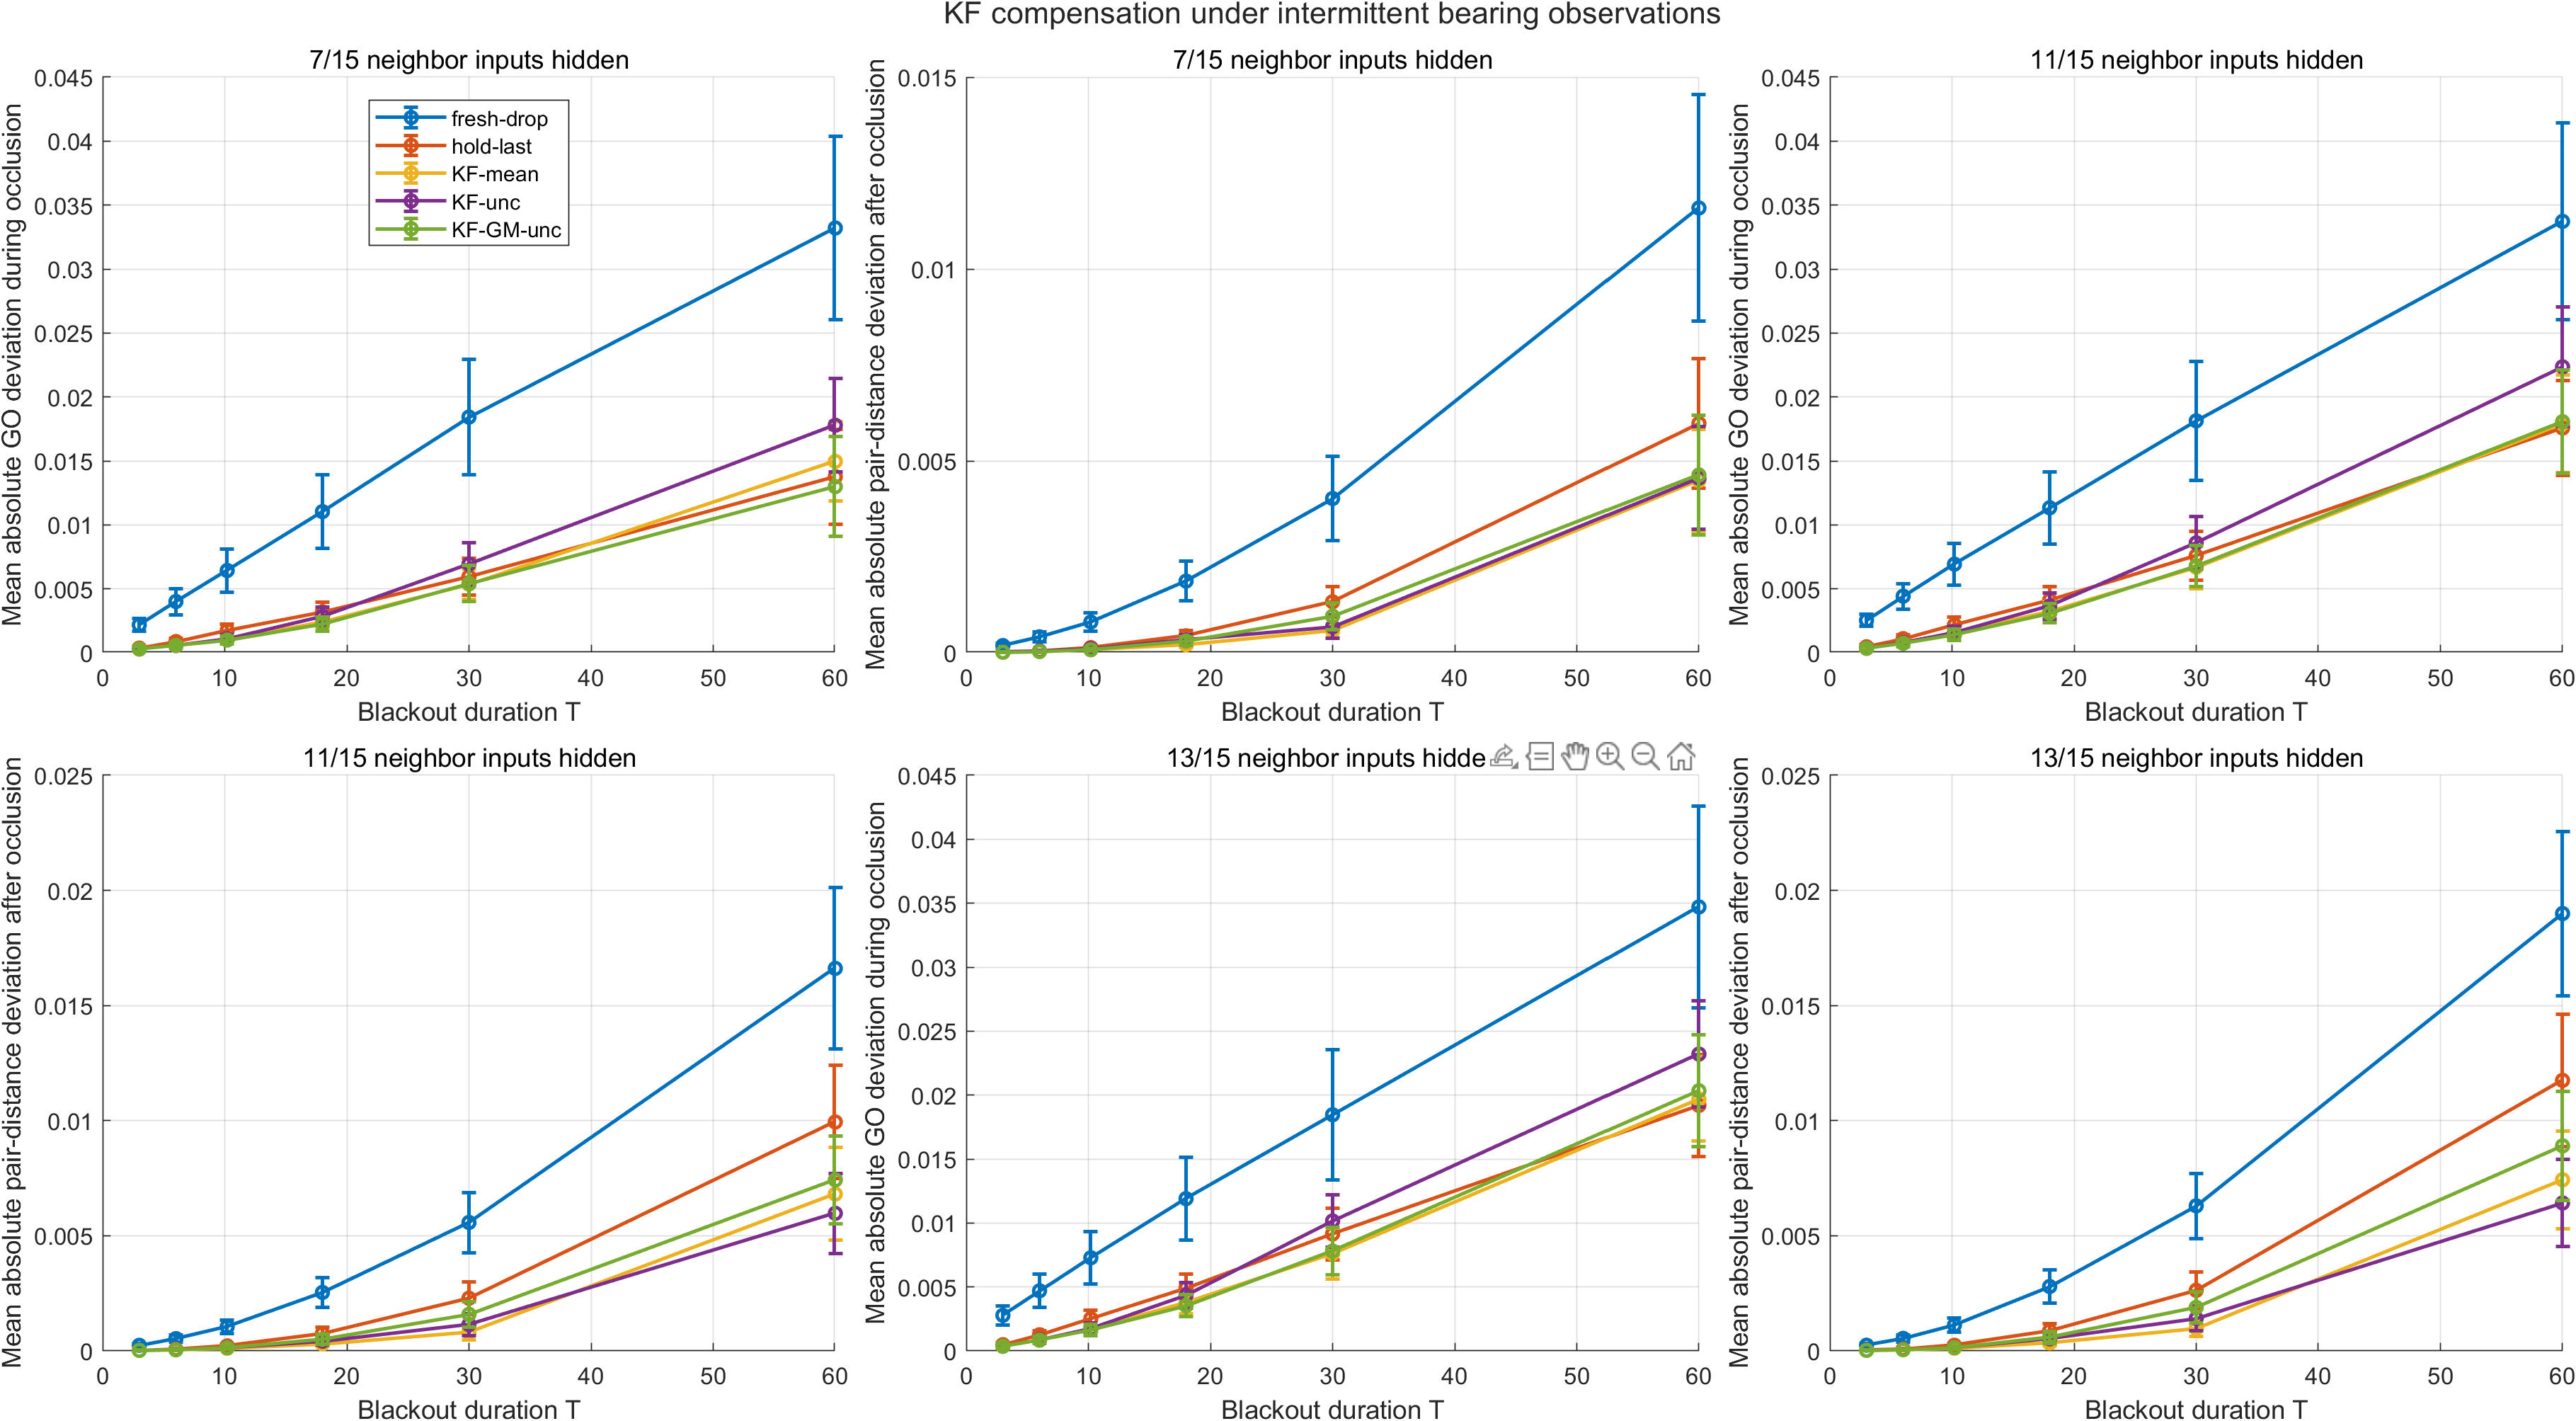
\includegraphics[width=0.98\linewidth]{kf-performance-summary.png}
 \caption{不同遮挡强度和时长下的绝对 GO 偏差与遮挡后距离偏差。图中旧误差线为种子均值的近似区间；主比较以表中的配对 bootstrap 区间为准。}
 \label{fig:kf_performance}
\end{figure}

图~\ref{fig:kf_vs_hold} 直接给出各 Kalman 方法相对 hold-last 的配对差值。负值表示相对 hold-last 降低偏差。该图用于区分“保留旧方位已带来的收益”和“Kalman 外推或协方差卷积额外带来的收益”：短时遮挡中多数 Kalman 增量很小，中时遮挡中 KF-mean 和 KF-GM 对 GO 有可见增益，而 KF-uncertainty 的优势主要体现在长时间遮挡后的凝聚结构。

\begin{figure}[!tbp]
 \centering
 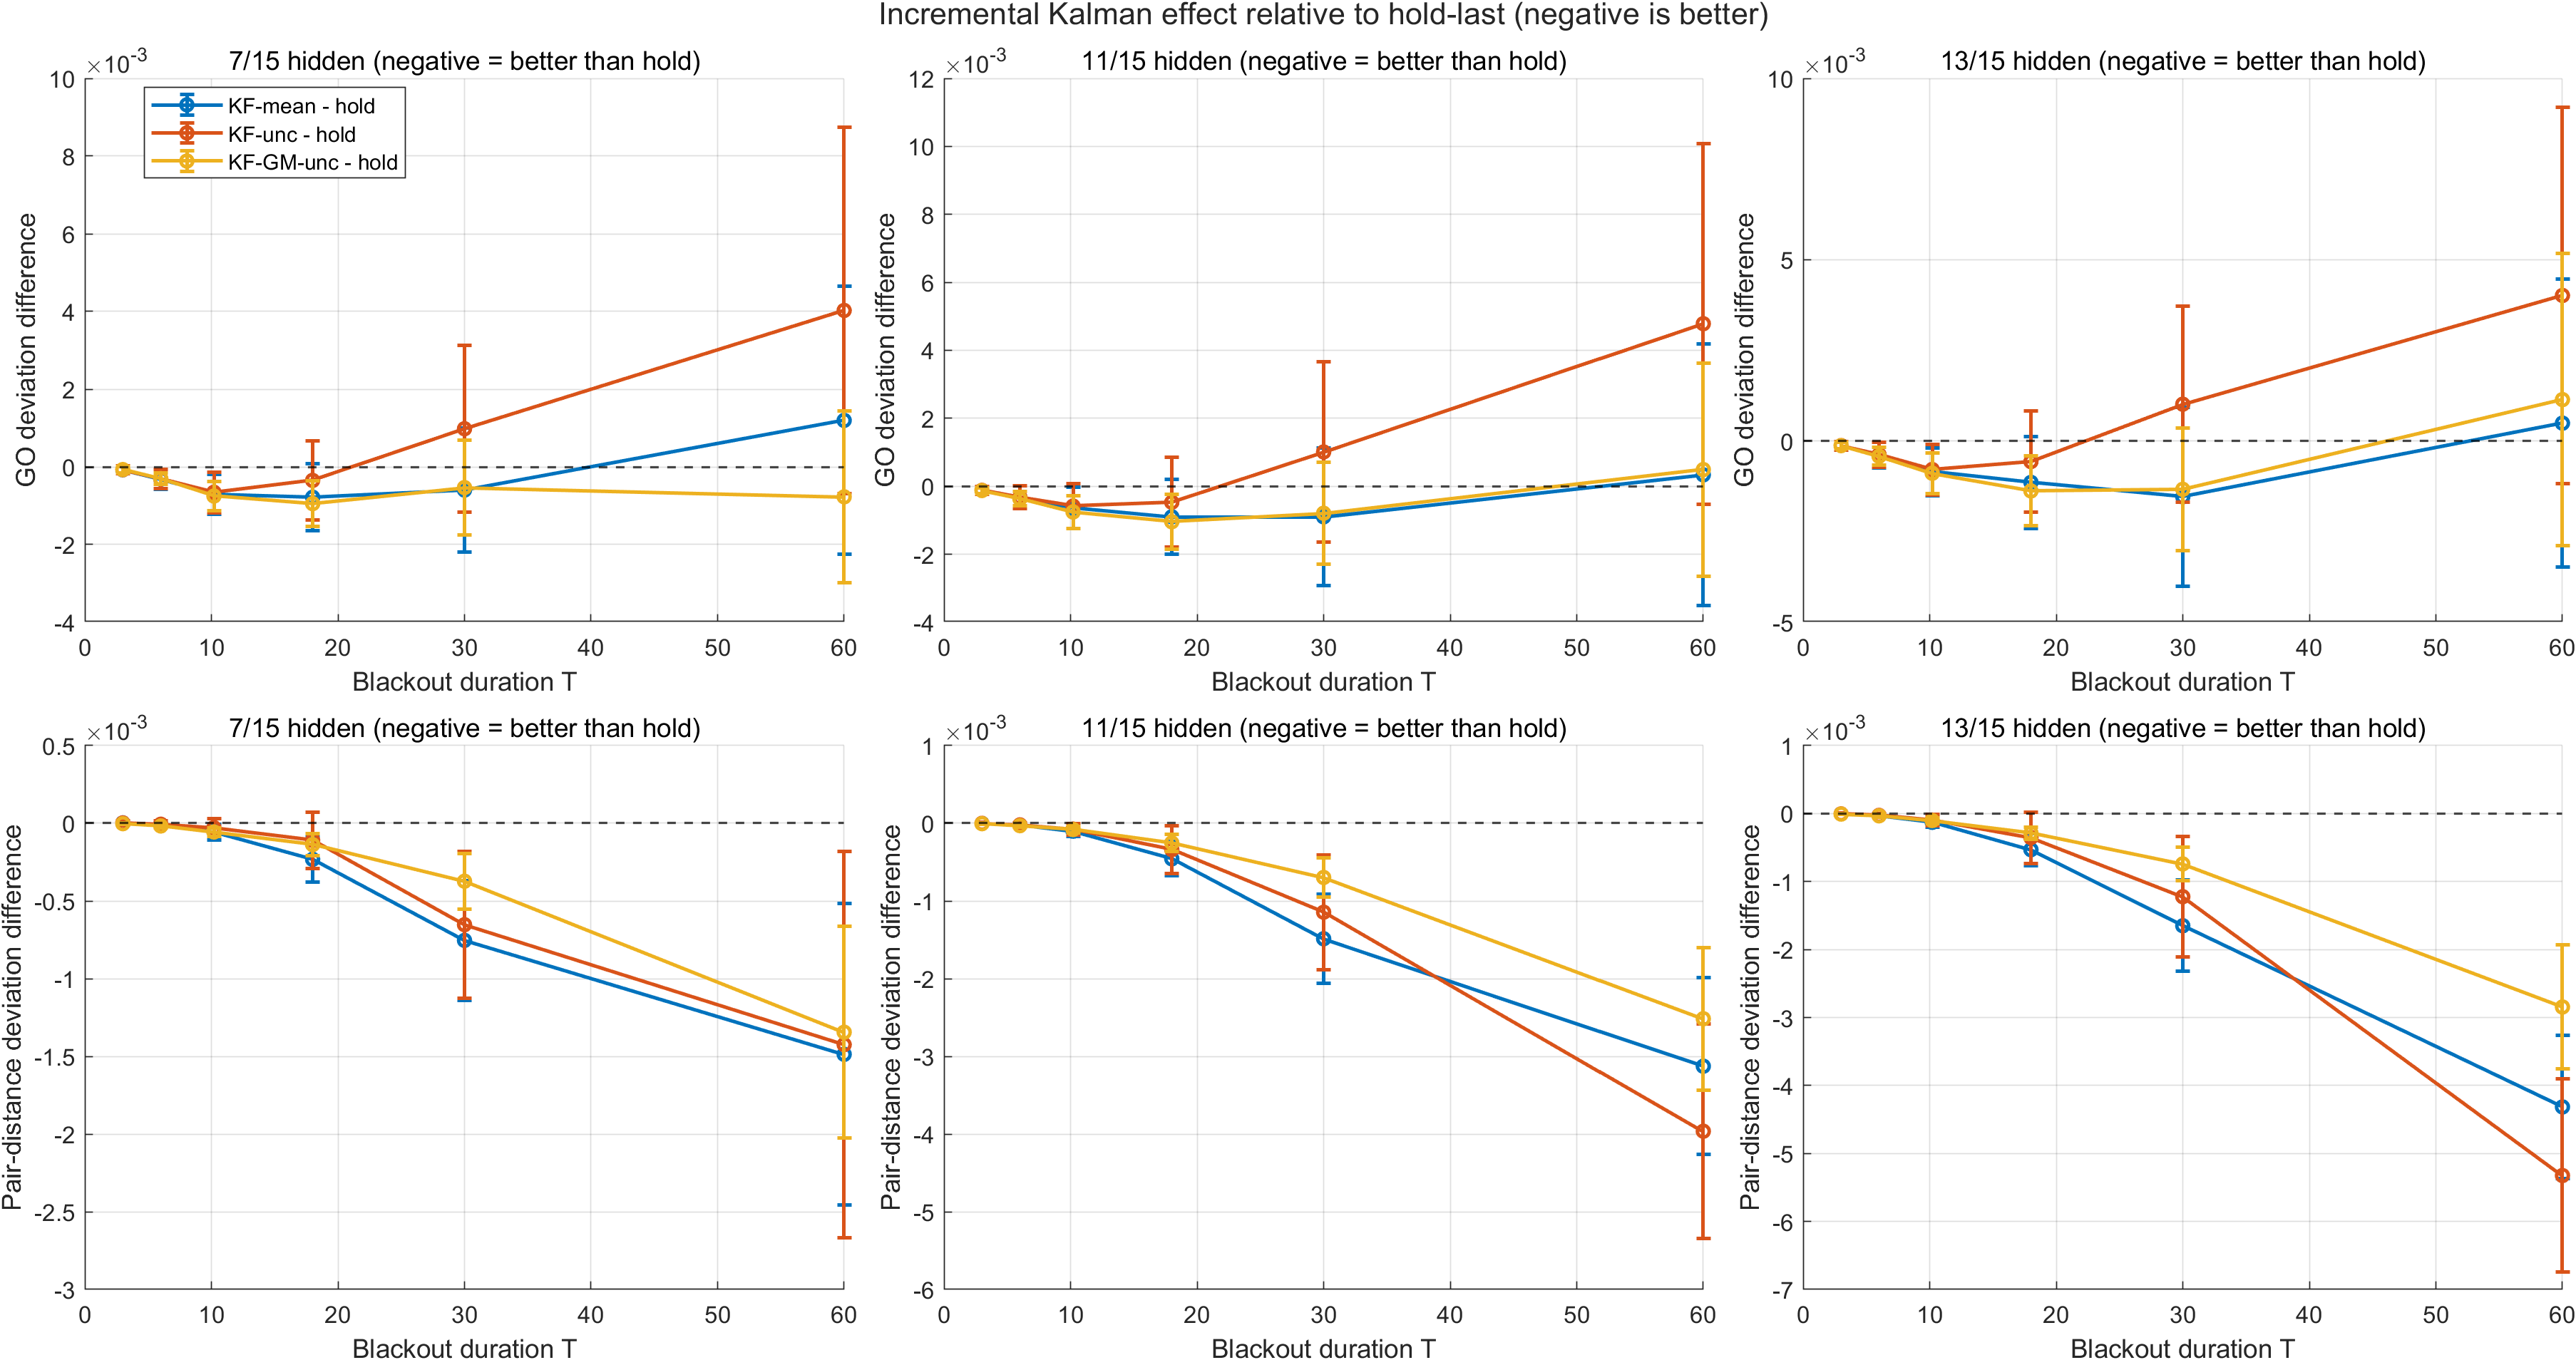
\includegraphics[width=0.98\linewidth]{kf-versus-hold.png}
 \caption{Kalman 方法相对 hold-last 的配对差值。横轴为遮挡时长，负值表示偏差低于 hold-last。}
 \label{fig:kf_vs_hold}
\end{figure}

\subsection{遮挡前受控转向与相对退化指标}

为检验动态方向变化中的预测补偿，本文设置受控转向干预。首先从同一无遮挡检查点分叉；在遮挡开始前 $20$ 步（$6$ 个模型时间单位），对编号为 $1$--$3$ 的领航个体施加幅值 $0.08$ 的异中心旋转方向输入，领航方向以 $0.025$ rad/模型时间的角速度缓慢变化。遮挡在第 $201$ 步开始，期间领航个体继续转向；其余个体通过邻居方位输入跟随。Kalman 轨迹在遮挡前接收连续变化的方位观测并估计方位角速度，遮挡开始时跟随者仍处于向新共同方向调整的过程中。

受控转向实验仍比较 fresh-drop、hold-last、KF-mean、KF-uncertainty 和 KF-GM-uncertainty。每个方法与同一转向任务下的无遮挡控制轨迹配对。除绝对 GO、LO 和凝聚距离外，定义相对退化指标
\begin{equation}
 D_{\mathrm{GO}}^{\mathrm{rel}}=
 \frac{\operatorname{mean}_{k\in\mathcal K_o}
 |GO_{\mathrm{method}}(k)-GO_{\mathrm{control}}(k)|}
 {\operatorname{mean}_{k\in\mathcal K_o}|GO_{\mathrm{control}}(k)|},
\end{equation}
并以相同方式定义 $D_{\mathrm{LO}}^{\mathrm{rel}}$ 和遮挡后凝聚距离相对偏差 $D_{\mathrm{pair}}^{\mathrm{rel}}$。这些指标比较的是观测缺失造成的相对退化，而不是不同模型本来具有的绝对性能差异。

图~\ref{fig:turn_timeline} 给出干预时序。图~\ref{fig:turn_relative} 给出完整 $30$ 个种子在 $11/15$ 条有向边隐藏条件下的统计结果。以 $T=3$ 和 $T=10.2$ 为例，fresh-drop 的相对 GO 退化分别为 $0.99\%$ 和 $2.82\%$，KF-GM-uncertainty 分别为 $0.13\%$ 和 $0.45\%$；对应的遮挡后相对凝聚距离偏差分别为 $0.127\%$ 和 $0.605\%$，KF-GM-uncertainty 分别降至 $0.0085\%$ 和 $0.090\%$。这些数值描述受控转向下各分支相对参考的偏差；未以目标航向误差或响应滞后验证转向跟随能力，也未将有转向和无转向的差异作为独立干预效应检验。图中区间为 $30$ 个种子间的近似 $95\%$ 区间，属于逐条件描述。

\begin{figure}[!tbp]
 \centering
 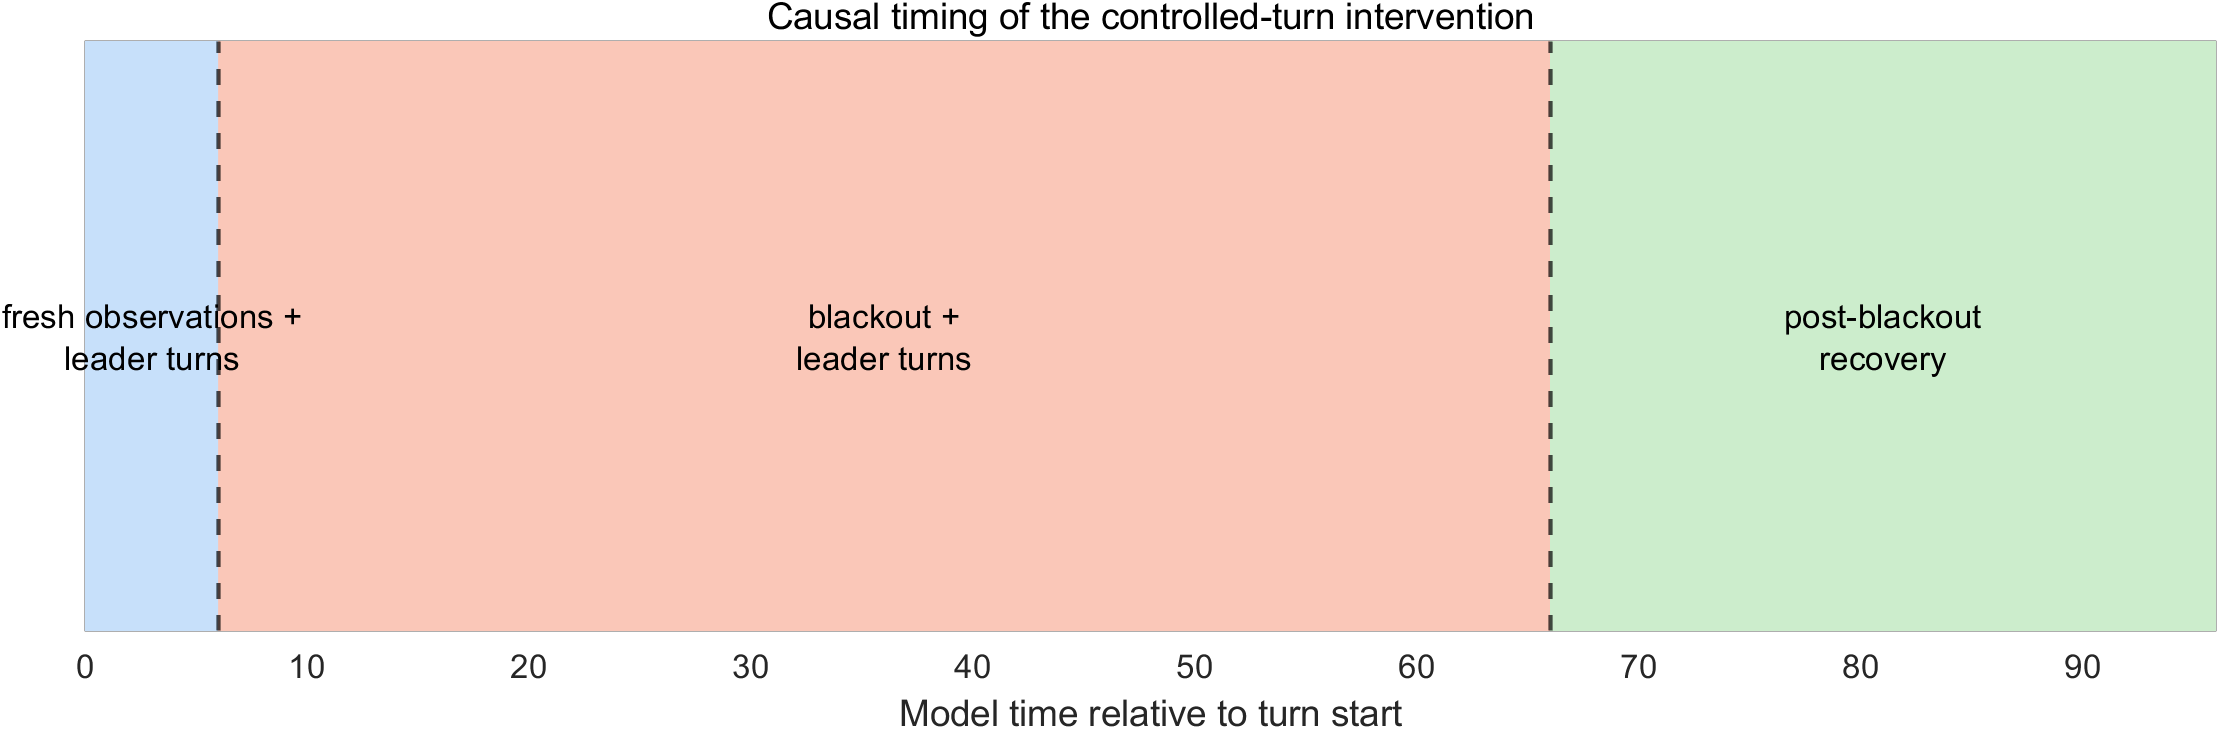
\includegraphics[width=0.82\linewidth]{intervention-timeline.png}
 \caption{受控转向实验时序：遮挡前先开始领航转向，随后进入连续遮挡和恢复窗口。}
 \label{fig:turn_timeline}
\end{figure}

\begin{figure}[!tbp]
 \centering
 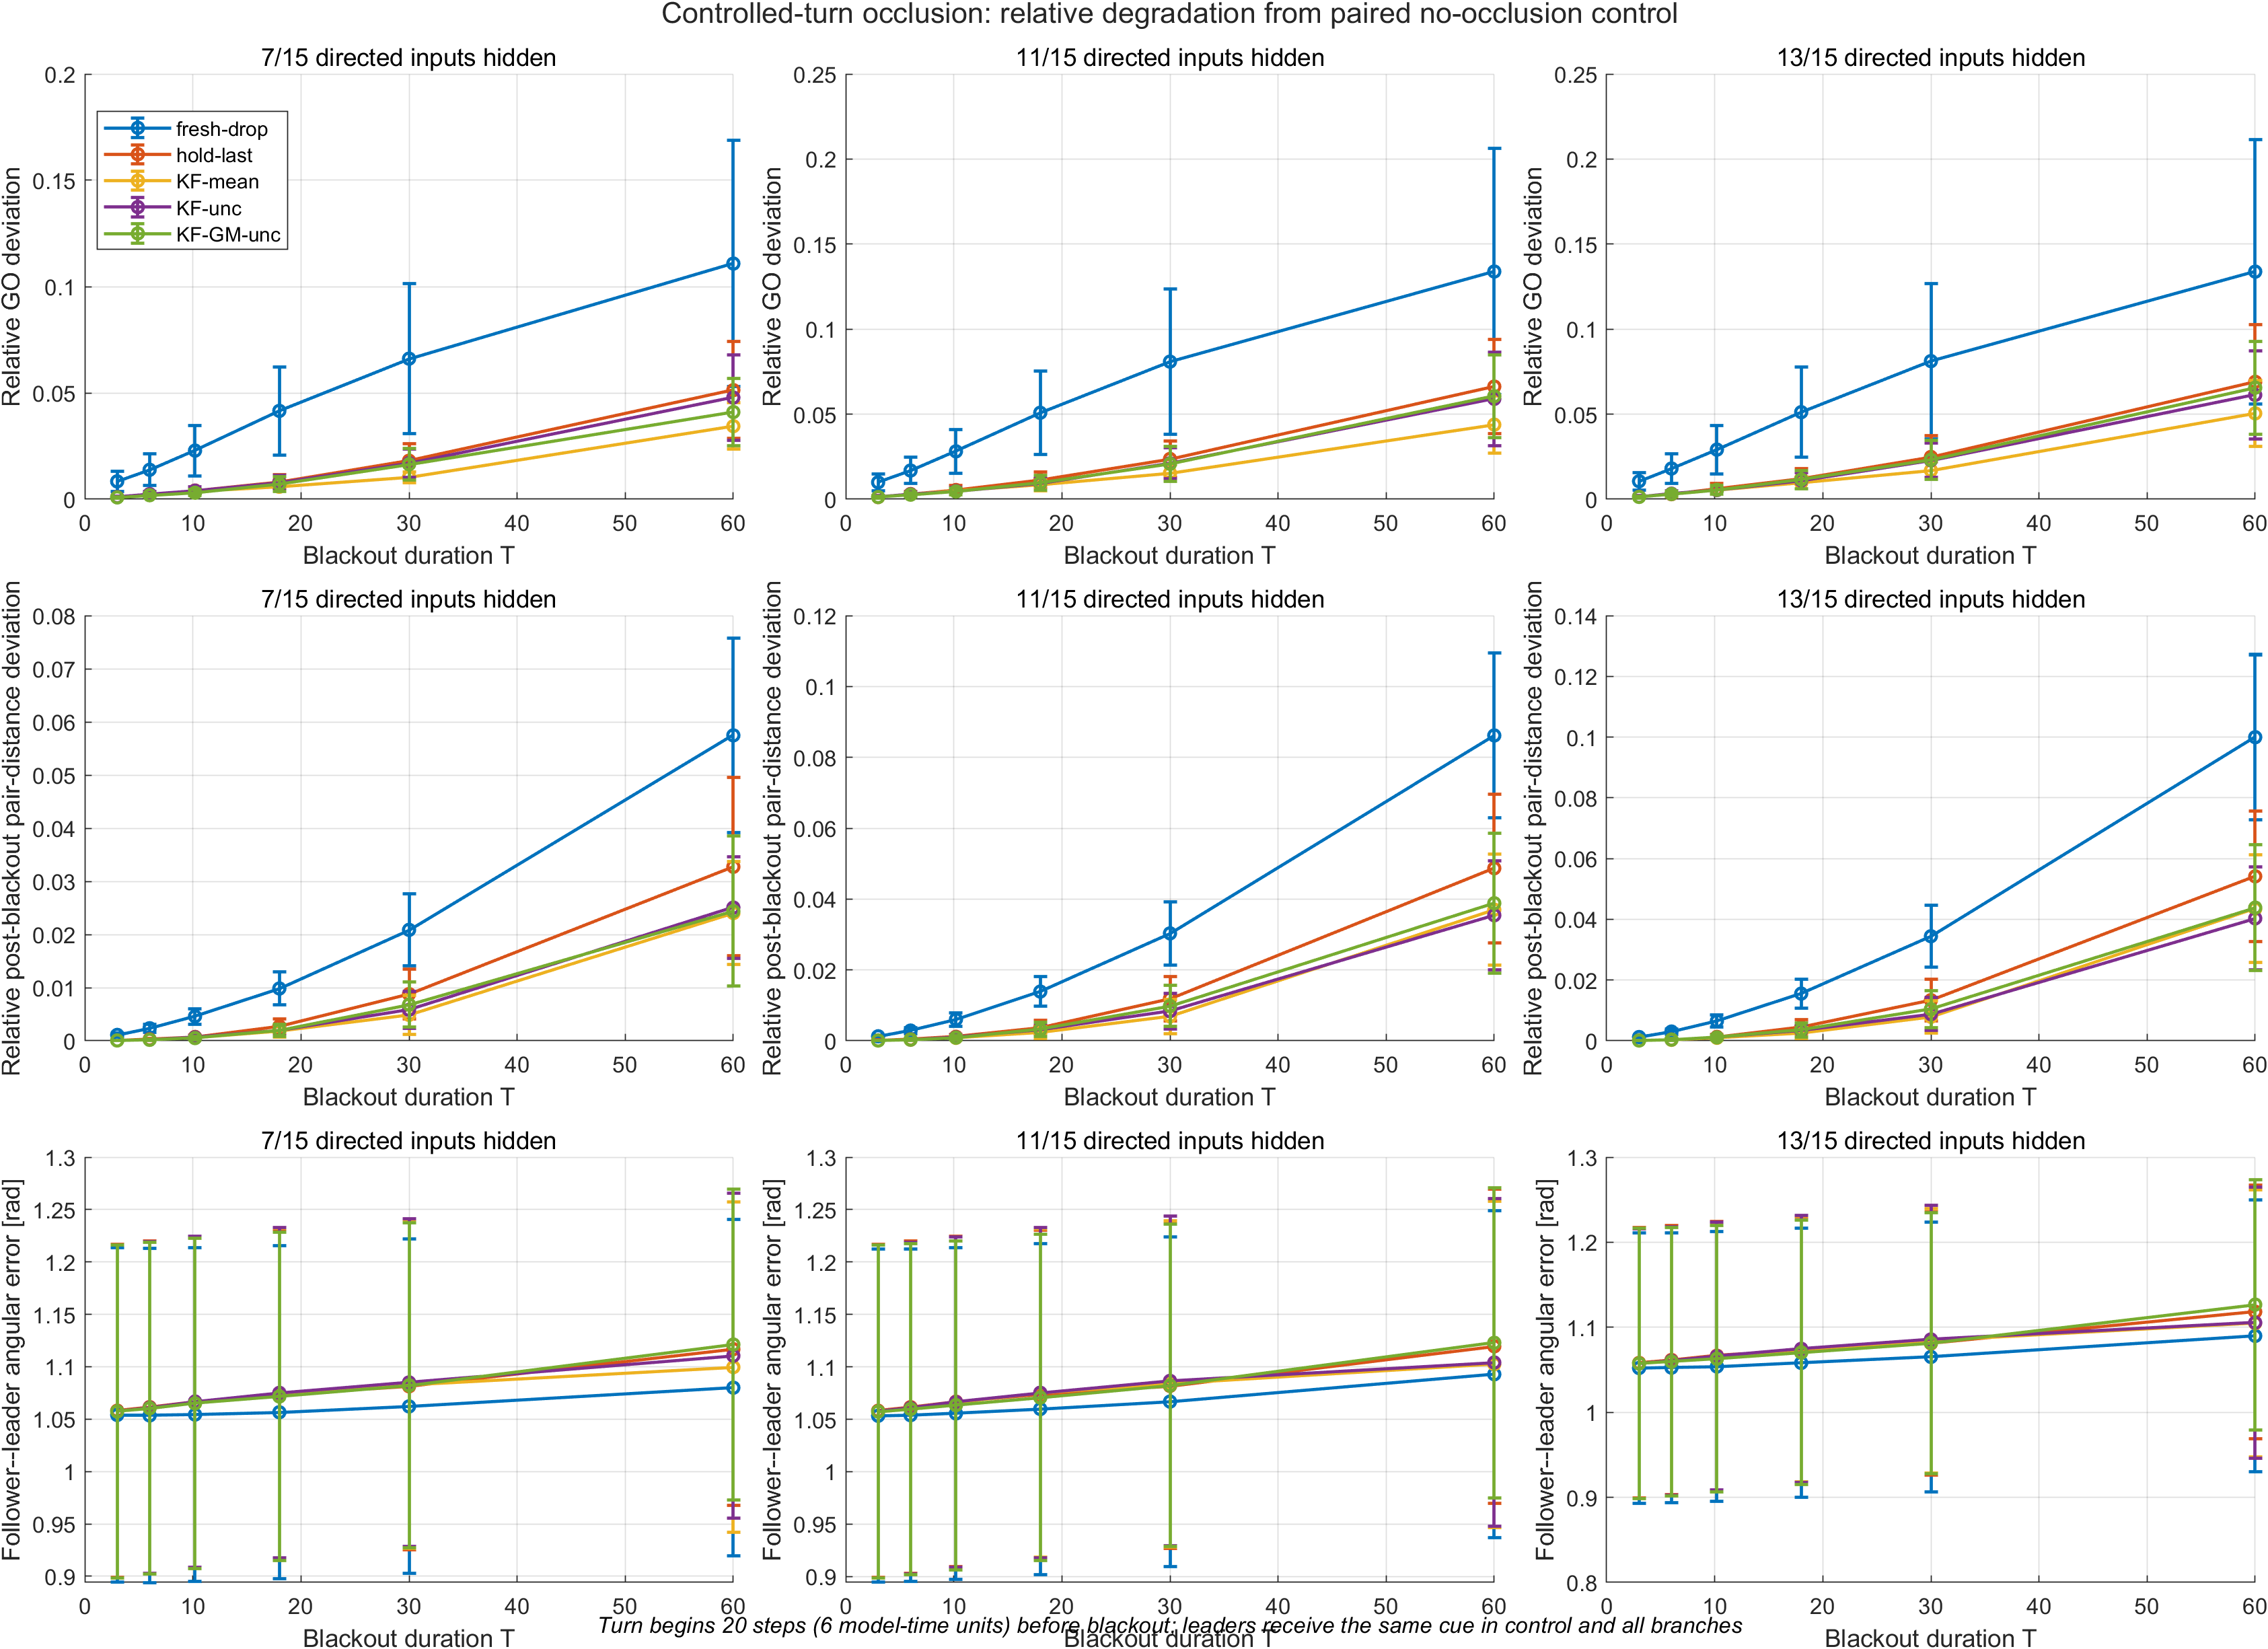
\includegraphics[width=0.98\linewidth]{relative-degradation.png}
 \caption{受控转向下相对无遮挡控制的退化（完整 $30$ 个种子）。误差线为种子间近似 $95\%$ 置信区间。}
 \label{fig:turn_relative}
\end{figure}

\subsection{不同感知模型的辅助结果及可比性}

Vicsek、Boids 和 Olfati--Saber 型规则分别使用邻居航向或相对位置等信息\upcite{Vicsek1995,Reynolds1987,OlfatiSaber2006}，与本文仅方位输入不同。其参数未作独立优化，控制器动力学与输入维度也不同，因此表~\ref{tab:mainstream} 只保留探索性的有序度与最小距离，不能视为性能上界或同信息条件下的算法排名。结果来自种子 $101$--$105$、$T=30$、隐藏 $7/15$ 条输入。

\begin{table}[!tbp]
\centering\small
\caption{不同感知条件的描述性参考。GO 损失为配对无遮挡值减遮挡值；最小距离按全仿真记录统计。$n=5$，仅报告既有均值，不作显著性排名。}
\label{tab:mainstream}
\begin{tabular}{lrrr}
\toprule 模型 & 遮挡期 GO & GO 损失 & 最小距离$/L$\\\midrule
本文 KF-unc & 0.729 & $-0.0014$ & 0.00056\\
Vicsek（航向） & 1.000 & 0 & 0.00760\\
Boids（位置与航向） & 0.975 & 0.0038 & 0.00773\\
Olfati--Saber 型（位置与航向） & 0.911 & 0.0368 & 0.00764\\\bottomrule
\end{tabular}
\end{table}

历史实现的控制努力存在单位与角度回绕处理不一致，危险接近占比的采样窗口也分别包含 $601$ 与 $600$ 帧，因此本稿撤下相应跨模型排名及原比较图。历史危险阈值为 $10=0.01L$，事件是任意一对个体距离严格小于该阈值，不能解释为物理碰撞率。最小距离与时间平均有序度均不提供避碰保证；本稿也不据此声称更低控制代价。

\subsection{实验条件与后续验证}

上述闭环结果来自固定邻居身份、等权输入和脚本化连续遮挡条件；阻尼模型参数在前期开发阶段选定，新种子闭环评估沿用这些参数。下一步将以预测区间的实际覆盖率校准协方差，并扩展到动态邻居集合和真实几何遮挡。数据关联、邻居存在概率和碰撞约束需要相应的估计与控制模块。

\section{讨论与限制}

\paragraph{经验描述量的价值与范围}
指数加权量在既有局部回放中比总幅值基准更能描述纵向响应，但其正值累加、左右对称和固定 $\kappa$ 限制了可表达的方向信息。前两组实验属于定义和实现检查，第三组属于开发性关联分析。投稿前需要加入加权余弦、圆周合矢量等方向基线，以及在独立动态群体数据上的检验，才能判断该量是否提供超出常用低阶特征的价值。

\paragraph{输入重建不等于稳定的预测或闭环优势}
五种子中心条件的输入误差下降与方位 RMSE 汇总反转同时存在，说明核叠加误差不能由单一角误差指标替代。恢复首步 NIS 和覆盖率表明近似后验失配；因此连续卷积的理想 MMSE 性质不能作为当前滤波器校准正确的证据。扩展实验的 $T=60$ 常角速度预测诊断还受到激活门控筛选，必须在共同边与共同时间窗上重新评价。闭环偏差较小表示更接近 fresh，尚未证明转向跟踪、碰撞风险或任务性能改善。

\paragraph{尚缺的消融与外推验证}
需要完整的 CV/GM 与 mean/uncertainty 因子组合、固定核展宽和简单角速度外推基线，并同时记录激活边数量与停注时长。当前仅采用 $N=20$、固定身份、二维周期区域和脚本化缺失；动态邻居、几何遮挡、朝向误差、数据关联、运动约束与显式避碰均未验证。现有种子已经用于开发与审阅，后续应在冻结指标、参数和排除规则后使用未检查数据；不能将新的数据分析直接升级为确认性实验。

\section{结论}

本文构建了历史方位预测到异中心神经场输入的接口，并以局部响应、同状态重建和检查点闭环三个层次评价。指数经验量较总幅值基准降低局部留组预测 RMSE $16.1\%$，该结论限于现有静态回放。五种子中心条件中，KF-mean 相对 hold 的同状态输入误差降低 $61.8\%$；方位 RMSE 的逐种子平均降低 $26.4\%$，但合并平方误差后增高 $13.5\%$，且逐种子配对差区间跨零，不能主张稳定的方位预测优势。

在三十种子扩展实验中，补偿在所测条件下降低相对 drop 的参考偏差，但相对 hold 的增量依赖缺失时长和指标。理论给出指定后验下的重建性质及实际输入差驱动的有限时间扰动界；由于后验失配和未封闭的几何反馈，它不提供集群稳定性或安全保证。当前工作属于探索性接口研究，后续重点是协方差校准、共同窗口诊断、完整消融和冻结方案后的独立验证。

\section*{数据与复现说明}
本稿修订不新增仿真，各结果批次分别对应下列目录：
\begin{itemize}[nosep,leftmargin=2em]
\item 局部经验量：\texttt{sq1-exponential-input-v1-r2}；
\item 五种子机制实验：\texttt{pilot\_seed1to5\_v1}；
\item 扩展缺失时长：\texttt{paper-kf-extended-v3/full}；
\item 受控转向：\texttt{turn-occlusion-pilot-v1/full}。
\end{itemize}
仓库基准为 \texttt{2ba7da1}。本次采用的汇总 CSV、实际工作区代码及图表的 SHA256、独立复算和编译记录保存在配套审稿目录；其中未跟踪开发包以文件哈希标识，不能仅由基准提交恢复。五种子共享包的原始 MAT 未包含在本次可用材料中，因此独立统计复核基于 CSV，未重放原始仿真。

\begin{thebibliography}{99}
\small
\setlength{\itemsep}{2pt}
\bibitem{Bai2024} C. Bai, P. Yan, H. Piao, W. Pan, and J. Guo, ``Learning-based multi-UAV flocking control with limited visual field and instinctive repulsion,'' \emph{IEEE Transactions on Cybernetics}, vol. 54, no. 1, pp. 462--475, 2024, doi: 10.1109/TCYB.2023.3246985.
\bibitem{Boldrer2026} M. Boldrer, V. Kratky, V. Walter, and M. Saska, ``Distributed Lloyd-based algorithm for uncertainty-aware multi-robot under-canopy flocking,'' \emph{IEEE Robotics and Automation Letters}, vol. 11, no. 5, pp. 5526--5533, 2026, doi: 10.1109/LRA.2026.3673985.
\bibitem{LiFlocking2024} C. Li, Y. Yang, T.-Y. Huang, and X.-B. Chen, ``An improved flocking control algorithm to solve the effect of individual communication barriers on flocking cohesion in multi-agent systems,'' \emph{Engineering Applications of Artificial Intelligence}, vol. 137, art. 109110, 2024, doi: 10.1016/j.engappai.2024.109110.
\bibitem{OlfatiSaber2006} R. Olfati-Saber, ``Flocking for multi-agent dynamic systems: algorithms and theory,'' \emph{IEEE Transactions on Automatic Control}, vol. 51, no. 3, pp. 401--420, 2006, doi: 10.1109/TAC.2005.864190.
\bibitem{Reynolds1987} C. W. Reynolds, ``Flocks, herds and schools: A distributed behavioral model,'' in \emph{Proceedings of SIGGRAPH '87}, pp. 25--34, 1987, doi: 10.1145/37401.37406.
\bibitem{Vicsek1995} T. Vicsek, A. Czirók, E. Ben-Jacob, I. Cohen, and O. Shochet, ``Novel type of phase transition in a system of self-driven particles,'' \emph{Physical Review Letters}, vol. 75, no. 6, pp. 1226--1229, 1995, doi: 10.1103/PhysRevLett.75.1226.
\bibitem{Salahshour2025} M. Salahshour and I. D. Couzin, ``Allocentric flocking,'' \emph{Nature Communications}, vol. 16, art. 9051, 2025, doi: 10.1038/s41467-025-64676-5.
\bibitem{Sinopoli2004} B. Sinopoli, L. Schenato, M. Franceschetti, K. Poolla, M. I. Jordan, and S. S. Sastry, ``Kalman filtering with intermittent observations,'' \emph{IEEE Transactions on Automatic Control}, vol. 49, no. 9, pp. 1453--1464, 2004, doi: 10.1109/TAC.2004.834121.
\bibitem{Xiourouppa2025} A. H. Xiourouppa, D. Mikhin, M. Humphries, and J. Maclean, ``Theoretical insights for bearings-only tracking in log-polar coordinates,'' \emph{IEEE Transactions on Aerospace and Electronic Systems}, vol. 61, no. 4, pp. 8534--8545, 2025, doi: 10.1109/TAES.2025.3547317.
\bibitem{Zhang1996} K. Zhang, ``Representation of spatial orientation by the intrinsic dynamics of the head-direction cell ensemble: a theory,'' \emph{The Journal of Neuroscience}, vol. 16, no. 6, pp. 2112--2126, 1996, doi: 10.1523/JNEUROSCI.16-06-02112.1996.
\bibitem{Krongauz2024} D. L. Krongauz, A. Ayali, and G. A. Kaminka, ``Vision-based collective motion: a locust-inspired reductionist model,'' \emph{PLOS Computational Biology}, vol. 20, no. 1, art. e1011796, 2024, doi: 10.1371/journal.pcbi.1011796.
\bibitem{Li2024} K. Li, L. Li, R. Gross, and S. Zhao, ``A collective perception model for neighbor selection in groups based on visual attention mechanisms,'' \emph{New Journal of Physics}, vol. 26, no. 1, art. 012001, 2024, doi: 10.1088/1367-2630/ad1b81.
\bibitem{Xue2025} K. Xue, D. Kong, P. Wang, Z. Xu, and Z. Huang, ``Attention-based selective interaction model for self-organized collective motion,'' \emph{Chaos, Solitons \& Fractals}, vol. 201, art. 117320, 2025, doi: 10.1016/j.chaos.2025.117320.
\end{thebibliography}
\end{document}
